              
%%%%%%%%%%%%%%%%%%%%%%%%%%%%%%%%%%%%%%%%%
% University Assignment Title Page 
% LaTeX Template
% Version 1.0 (27/12/12)
%
% This template has been downloaded from:
% http://www.LaTeXTemplates.com
%
% Original author:
% WikiBooks (http://en.wikibooks.org/wiki/LaTeX/Title_Creation)
%
% License:
% CC BY-NC-SA 3.0 (http://creativecommons.org/licenses/by-nc-sa/3.0/)
% 
% Instructions for using this template:
% This title page is capable of being compiled as is. This is not useful for 
% including it in another document. To do this, you have two options: 
%
% 1) Copy/paste everything between \begin{document} and \end{document} 
% starting at \begin{titlepage} and paste this into another LaTeX file where you 
% want your title page.
% OR
% 2) Remove everything outside the \begin{titlepage} and \end{titlepage} and 
% move this file to the same directory as the LaTeX file you wish to add it to. 
% Then add \input{./title_page_1.tex} to your LaTeX file where you want your
% title page.
%
%%%%%%%%%%%%%%%%%%%%%%%%%%%%%%%%%%%%%%%%%
\title{Modelagem Matemática da Propagação de Ondas em
Meios Não Homogêneos}
%----------------------------------------------------------------------------------------
%   PACKAGES AND OTHER DOCUMENT CONFIGURATIONS
%----------------------------------------------------------------------------------------

\documentclass[12pt, a4paper]{report}
% Importando pacotes básicos
% Codificação
\usepackage[utf8]{inputenc}
% Linguagem
\usepackage[brazil]{babel}
% Fonte
\usepackage[T1]{fontenc}
% Determinando as margens do documento
\usepackage[left=3cm, right=2cm, bottom=2cm, top=3cm]{geometry}
% Possibilita o uso de LINKs e URLs ao longo do documento
\usepackage[pdftex, hidelinks]{hyperref}
% possibilita o uso do simbolo de graus 
\usepackage{gensymb}

% Pacotes que não lembro a funcionalidade
\usepackage{setspace}
\usepackage{graphicx} % Uso de figuras (ACHO)
\usepackage{float}
\usepackage{mathptmx}
\usepackage{amsmath}

% Permitir quebra de página nos ambientes de equações
\allowdisplaybreaks

% Acho que usei isso para colocar figuras em tabelas
\usepackage{subfig}

% Anexar PDFs no LaTeX
\usepackage[final]{pdfpages}

% Para colocar apêndices no LaTeX
\usepackage[toc,page]{appendix}

% Insercao de codigos no LaTeX
\usepackage{listings}
\lstset{language=Python}    % Setando a linguagem padrao

\usepackage{color}

\definecolor{codegreen}{rgb}{0,0.6,0}
\definecolor{codegray}{rgb}{0.5,0.5,0.5}
\definecolor{codepurple}{rgb}{0.58,0,0.82}
\definecolor{backcolour}{rgb}{0.95,0.95,0.92}

% Definindo estilo de exibição de código
\usepackage{color}
\lstdefinestyle{mystyle}{
	backgroundcolor=\color{backcolour},   
	commentstyle=\color{codegreen},
	keywordstyle=\color{magenta},
	numberstyle=\tiny\color{codegray},
	stringstyle=\color{codepurple},
	basicstyle=\footnotesize,
	breakatwhitespace=false,         
	breaklines=true,                 
	captionpos=b,                    
	keepspaces=true,                 
	numbers=left,                    
	numbersep=5pt,                  
	showspaces=false,                
	showstringspaces=false,
	showtabs=false,                  
	tabsize=4,
	basicstyle=\scriptsize
}

% Para adicionar notas e TODO's
\usepackage{todonotes}

% Para colocar margem da na legenda de um figure/table
% \usepackage[margincaption,outercaption,ragged,wide]{sidecap}
% \sidecaptionvpos{figure}{t} 
\usepackage[figurename=Fig.]{caption}
\DeclareCaptionStyle{figstyle}
  [format=plain,margin=0pt,justification=centering]
  {format=hang,calcmargin={0pt,\widthof{\captionfont\captionlabelfont\figurename~\thefigure: }},
   font=small,labelfont=bf}
\captionsetup[figure]{style=figstyle}

% Indenta o primeiro parágrafo das seções
\usepackage{indentfirst}

% Translating mathematical function names to Portuguese
\let\sin\relax        \DeclareMathOperator{\sin}{sen}
\let\arcsin\relax     \DeclareMathOperator{\arcsin}{arcsen}

\begin{document}

\begin{titlepage}

\newcommand{\HRule}{\rule{\linewidth}{0.5mm}} % Defines a new command for the horizontal lines, change thickness here

\center % Center everything on the page
 
%----------------------------------------------------------------------------------------
%   HEADING SECTIONS
%----------------------------------------------------------------------------------------

\textsc{\LARGE Centro Federal de Educação Tecnológica de Minas Gerais}\\[3.5cm] % Name of your university/college
\textsc{\Large Engenharia de Computação}\\[3.5cm] % Major heading such as course name

%----------------------------------------------------------------------------------------
%   TITLE SECTION
%----------------------------------------------------------------------------------------

\HRule \\[0.4cm]
{ \huge \bfseries Modelagem Matemática da Propagação de Ondas em Meios Não Homogêneos}\\[0.4cm] % Title of your document
\HRule \\[2.5cm]
 
%----------------------------------------------------------------------------------------
%   AUTHOR SECTION
%----------------------------------------------------------------------------------------

\begin{minipage}{0.4\textwidth}
\begin{flushleft} \large
\emph{Orientando:}\\ Marcelo Lopes de Macedo \textsc{Ferreira Cândido} % Your name
\end{flushleft}
\end{minipage}
~
\begin{minipage}{0.4\textwidth}
\begin{flushright} \large
\emph{Orientador:} \\
Prof. Dr. Luis Alberto \textsc{D'Afonseca} % Supervisor's Name
\end{flushright}
\end{minipage}\\[7cm]

% If you don't want a supervisor, uncomment the two lines below and remove the section above
%\Large \emph{Author:}\\
%John \textsc{Smith}\\[3cm] % Your name

%----------------------------------------------------------------------------------------
%   DATE SECTION
%----------------------------------------------------------------------------------------

{\large BELO HORIZONTE\\\today}\\[1cm] % Date, change the \today to a set date if you want to be precise

%----------------------------------------------------------------------------------------
%   LOGO SECTION
%----------------------------------------------------------------------------------------

%\includegraphics{logo.png}\\[1cm] % Include a department/university logo - this will require the graphicx package
 
%----------------------------------------------------------------------------------------

\vfill % Fill the rest of the page with whitespace

\end{titlepage}


    \lstset{style=mystyle}

    \tableofcontents
    
    \chapter{Introdução}

    O ser humano interage e necessita interagir com ondas a todo momento. Essas pertubações mecânicas ou eletromagnéticas fazem parte do nosso cotidiano desde o nosso acordar, pela luz (um tipo de onda eletromagnética) que é emitida/refletida até nós e que nos permite observar o mundo ao nosso redor pelos nossos olhos ou pelo som (composto por ondas mecânicas) emitido por carros, fábricas, choro de crianças ou um belo canto de pássaros que são captados por nossos ouvidos. Interagimos com as ondas até indiretamente, como o leitor agora interage, por exemplo, ou estando sentado em uma cadeira ou andando sobre um calçado ou se deslocando em algum meio de transporte, que provavelmente tem algum mineral adquirido através de estudos sismológicos, que utilizam massivamente os conceitos de ondulatória.
    
    Na área da Geologia (e também na Medicina, Física, construção civíl, por exemplo), aplicam-se, pelo menos, dois métodos para o estudo de fenômenos ondulatórios e de estruturas geológicas não homogêneas: o \textbf{método de diferenças finitas} e o \textbf{traçamento de raios}. Utiliza-se esses métodos (principalmente o segundo) na busca por minérios e pela história da formações de estruturas geológicas.
    
    Neste trabalho, objetivamos comparar esses dois métodos numéricos computacionais na simulação da propagação de ondas através de meios não-homogêneos. Tal comparação se dará nos aspectos da dificuldade de implementação dos métodos, seus custos, sua intuitividade e qual seria a melhor área para a aplicação de tais métodos.
    
    Para alcançar tal objetivo, o autor deste relatório e orientando dessa iniciação científica passa por uma série de estudos prévios (Capítulos \ref{cap:cientComp}, \ref{cap:EDOs}, \ref{cap:aproxPVI}, \ref{cap:ond} e \ref{cap:EDPs}) que dão base ao estudo realizado nesse trabalho, para enfim abordar os métodos a serem comparados (Capítulos \ref{cap:MDF}, \ref{cap:RT} e \ref{cap:CompMDFeRT}).
    
    Os principais códigos desenvolvidos durante o projeto, bem como esse próprio relatório, podem ser encontrados no repositório do autor (\url{https://github.com/MarceloFCandido/PIC}). Os códigos envolvidos diretamente na comparação dos métodos também se encontram no apêndice desse relatório.
    
    \chapter{Uma Breve Introdução à Computação Científica}

    \label{cap:cientComp}

    A computação científica visa a resolução de problemas físicos, matemáticos, químicos, biológicos 
    ou de outra área da ciência utilizando-se o Cálculo Numérico executado por computadores. Essas resoluções
    são de cunho numérico (ou seja, não são analíticas) e obtidas através da elaboração e execução de algoritmos
    que modelam o problema a ser estudado. Esses algoritmos são executados por computadores e se baseiam em 
    operações aritméticas e lógicas, que são as únicas que um computador pode realizar \cite{fred}.

    \section{Soluções de Problemas}
    
        Segundo Campos \cite{fred}, a resolução de problemas se dá por meio de quatro etapas:
        \begin{enumerate}
            \item \textbf{definição do problema}: determina-se qual o problema a ser resolvido;
            \item \textbf{modelagem matemática}: obtém-se o modelo matemático do problema real por meio
            de uma formulação matemática;
            \item \textbf{solução numérica}: determina-se qual o método numérico a ser 
            utilizado para a resolução do problema modelado matemático. Implementa-se o método na forma de uma algoritmo, que, 
            após ser codificado em um programa, deve ser executado por um computador;
            \item \textbf{análise dos resultados}: avalia-se se a solução obtida é satisfatória para o problema. Caso 
            contrário, modela-se novamente o problema através de uma nova formulação matemática a fim de se 
            obter uma nova solução numérica.
        \end{enumerate}
    
    \section{Aritmética Computacional}
    
        Tudo o que um computador consegue entender são \textit{strings} (cadeias de caracteres) de zeros e uns. Cada um dos dos componentes dessas \textit{strings} é conhecido por \textit{bit}, que também pode ser definido como um dígito \textbf{binário}. Toda a matemática que um computador consegue realizar é baseada nessa representação. Por conta disso, um computador consegue representar a forma exata de alguns números racionais. Entretanto, os demais números são representados por aproximações. Como sabemos, a maior parte dos números desse tipo tem casas decimais e, para serem representados computacionalmente, precisam seguir um padrão específico \cite{burden}.
        
        Em 1985, o Instituto de Engenheiros Eletricistas e Eletrônicos (IEEE, em inglês) adotou o padrão técnico IEEE-754 para ponto flutuante, que é a forma pela qual um computador consegue representar números com casas decimais. Muitos fabricantes de microprocessadores adotaram esse padrão, que define um ponto flutuante como um ``real longo'' de 64 \textit{bits} na forma 
        \begin{equation*}
            (-1)^s\cdot 2^{c - 1023}(1 - f)
        \end{equation*}
        na qual $s$ é um indicador de sinal, $c$ é um expoente chamado de ``característica'' e $f$ é uma fração binária que recebe o nome de ``mantissa''. Na \text{string} de 64 \textit{bits}, $s$ recebe um \textit{bit}, $c$ recebe 11 e $f$ recebe 54 \textit{bits} \cite{burden}.
    
        O uso desse formato para a representação de números leva a erros de arredondamento em cálculos computacionais caso um dos números envolvidos nos cálculos não seja uma potência de dois. Isso ocorre por conta da representação numérica da máquina ser finita, o que leva a aproximações numéricas. Esse erro deve ser controlado para que não interfiram significativamente nos resultados dos cálculos \cite{burden, fred}.
        
    \section{Tipos de Erros Envolvidos na Solução de Problemas}
    
        Também segundo Campos \cite{fred}, existem pelo menos três tipos de erros que podem ser encontrados na solução de problemas (excetuando-se os erros grosseiros referidos pelo autor). São eles:
        \begin{enumerate}
            \item \textbf{erro de arredondamento e/ou truncamento}: a transformação de um número em seu correspondente em ponto flutuante pode se dar por 
            \begin{itemize}
                \item \textbf{arredondamento}: seja uma máquina com suporte a números de $k$ algarismos. Se ela receber um número $i$ de $k + n$ algarismos e o $(k + 1)$-ésimo algarismo for maior ou igual a $5$, soma-se $1$ ao $k$-ésimo algarismo e corta-se (trunca-se) os $n$ últimos algarismos de $i$. Caso o $(k + 1)$-ésimo algarismo for menor que $5$, realiza-se apenas o truncamento;
                \item \textbf{truncamento}: ainda considerando uma máquina como a do caso anterior, se ela receber um número $i$ de $k + n$ algarismos, ela truncará os últimos $n$ algarismos de $i$ \cite{burden};
            \end{itemize}
            \item \textbf{erro absoluto e erro relativo}: o erro absoluto é medido por \begin{equation}
                e_{\text{abs}} = v_{\text{real}} - v_{\text{aprox.}}
            \end{equation}
            onde $e_{\text{abs}}$ é o erro absoluto, $v_{\text{real}}$ é o valor real e $v_{\text{aprox.}}$ é o valor aproximado. Já o erro relativo é dado por
            \begin{equation}
                e_{\text{rel}} = \dfrac{v_{\text{real}} - v_{\text{aprox.}}}{v_{\text{real}}}
            \end{equation}
            onde $e_{\text{rel}}$ é o erro relativo, $v_{\text{real}}$ é o valor real e $v_{\text{aprox.}}$ é o valor aproximado \cite{fred}.
            \item \textbf{erro na modelagem}: em alguns problemas, é necessária a criação de uma expressão matemática na etapa de modelagem. Essa expressão é criada a partir de dados experimentais, que podem não estar próximos o bastante do problema real e, dessa forma, interferirem significativamente nos resultados. Com isso, torna-se necessária uma nova modelagem \cite{fred};
        \end{enumerate}
    

    \chapter{Equações Diferenciais Ordinárias}

    \label{cap:EDOs}

    \section{Definição e Características de Equações Diferenciais}
    
        Primeiramente, antes de definir uma equação diferencial ordinária, é necessário se definir e caracterizar uma equação diferencial. As equações diferenciais são, basicamente, aquelas cujas incógnitas são funções (variáveis dependentes) de uma variável independente, podendo envolver também algumas derivadas dessas funções.

        \subsection{A Ordem de uma Equação Diferencial}

            No mundo das equações diferenciais, a \textbf{ordem} da equação é 
            determinada pela derivada de maior ordem existente na equação. Ou seja, se
            em uma equação, na qual a incógnita é \(y\), a derivada de maior ordem
            da função-incógnita é \(y^{(n)}\), então a equação diferencial é de
            ordem \(n\). Para maior elucidação, temos por exemplo a equação
            \begin{equation*}
                y' + 3y = 0
            \end{equation*}
            que é dita de primeira ordem, pois a derivada de ordem mais alta, que está
            na equação, da função \(y\) é \(y'\), de ordem 1. Já no caso da equação
    
            \begin{equation*}
                y'' + 5y = y''' + 3t
            \end{equation*}
            a ordem é 3, pois a derivada de \(y\) com ordem mais alta na equação é
            \(y'''\).

        \subsection{Linearidade}

            Uma equação diferencial é dita \textbf{linear} quando todos os
            coeficientes que multiplicam as derivadas de \(y\) são funções da(s)
            variável(eis) independentes $a_{i}(t) \text{, com }i = 0, 1, ..., n$,
            não sendo essas funções da própria \(y\) ou uma de suas derivadas. Por exemplo:
            \(... + xy^{(i)} + \cdots\), sendo \(t\) a variável de \(y\). 
            
            A equação
            diferencial ordinária linear geral é
            \begin{equation}
                a_{n+1}(t)y^{(n)}(t) + a_{n}(t)y^{(n-1)}(t) + ... + a_{3}(t)y''(t) 
                + a_{2}(t)y'(t) + a_{1}(t)y(t) + a_{0} = f(t)
            \end{equation}
            Qualquer equação que saia desse padrão é dita \textbf{não-linear}.

        \subsection{Solução de uma Equação Diferencial Ordinária}

            Uma função $y(t)$ é dita solução de uma equação diferencial 
            se ela e suas respectivas derivadas estão definidas em determinado intervalo e 
            podem ser substituídas na equação sem ocorrer desigualdades \cite{regiIntro}. 
            Por exemplo, $y(t) = e^t$ é solução de
            \begin{equation}
                \label{exSol1}
                y' - y = 0
            \end{equation}
            pois $y'(t) = e^t$ e a subtração entre $y(t)$ e $y'(t)$ leva a um resultado nulo. 
            Em contrapartida, $y(t) = \cos{t}$ não pode ser solução de (\ref{exSol1}) pois a 
            função subtraída de sua derivada $y'(t) = -\sin{t}$ não leva a um resultado nulo.
    
    
    \section{A Definição de uma Equação Diferencial Ordinária}

        \label{defEDO}
        Uma Equação Diferencial Ordinária (EDO) é uma equação como
        \begin{equation}
            \label{EDOgeral}
            a_{n+1}y^{(n)}(t) + a_{n}y^{(n-1)}(t) + \cdots + a_{3}y''(t) + a_{2}y'(t) + a_{1}y(t) + a_{0} = f(t)
        \end{equation}
        sendo a função \(y(t)\) e suas derivadas \(y'(t)\), \(y''(t)\), ...,
        \(y^{(n-1)}(t)\) e \(y^{(n)}(t)\) as incógnitas da equação. Ou seja, a
        solução dessas equações são funções com \textbf{uma} variável
        independente (por isso é dita ordinária, se houvessem mais variáveis
        independentes a equação diferencial seria dita parcial, tipo que será
        tratado mais a frente) \cite{boyce9, regiIntro}.
    
    \section{Sistemas de Equações Diferenciais Lineares}
    
        Assim como existem sistemas de equações de $n$-ésimo grau, as equações diferenciais também podem ser agrupadas em sistemas como o abaixo
        \begin{equation}
            \begin{cases}
                y'_1(t) = a_1y_1(t) + b_1y_2(t)\\
                y'_2(t) = a_2y_2(t) + b_2y_1(t)
            \end{cases}
        \end{equation}
	    Mais a frente serão mostradas aplicações para esse tipo de sistema.
	        
    \section{Problema de Valor Inicial (PVI)}
        \label{PVIsec}
    
        Um problema de valor inicial (PVI) é dado por
        \begin{align}
            \label{PVIeq}
            y' = f(t)\\
            \label{PVIcond}
            y(t_0) = y_0
        \end{align}
        sendo (\ref{PVIeq}) uma equação diferencial ordinária e (\ref{PVIcond}) sua condição inicial, ou seja,
        como o sistema que (\ref{PVIeq}) descreve se encontrava no instante $t_0$, em geral consideramos que $t$ se 
        refere a tempo \cite{regiIntro}.
        
        Um PVI também pode ser descrito por um sistema de equações diferenciais ordinárias. Nesse caso, devem haver $n$ condições iniciais para cada uma das $n$ equações que formarem o sistema.
        
    \section{Problema de Valores de Contorno para Fronteiras com Dois Pontos (PVC)}
    
        Considere uma equação diferencial de segunda ordem como
        \begin{equation}
            y'' + p(t)y' + q(t)y = g(t)
        \end{equation}
        com as seguintes condições iniciais
        \begin{align}
            y(\alpha) &= y_0\\
            y(\beta) &= y_1
        \end{align}
        Esse tipo de problema é chamado \textbf{problema de valores de contorno com dois pontos} \cite{boyce9}. Esse tipo de problema costuma ser usado para descrição de situações espaciais em equilíbrio, ou seja, que não variam no tempo.
        
        
    \section{Aplicações das Equações Diferenciais Ordinárias}
        
        Por se tratarem de equações envolvendo taxas de variação, as EDO's são muito úteis para descrever situações físicas, químicas e biológicas. Alguns exemplos de situações nas quais esse tipo de equação é utilizado são 
        \begin{itemize}
            \item o modelo de crescimento populacional de Malthus;
            \item o carregamento e o descarregamento de um capacitor;
            \item a função logística criada por Verhulst;
            \item as equações presa-predador de Lotka-Volterra;
            \item os sistemas massa-mola;
            \item descrições de reações químicas.
        \end{itemize}
        
        Algumas dessas aplicações serão mais detalhadas no Capítulo \ref{cap:aproxPVI}, que também exporá exemplos de como podem ser resolvidas numericamente e os resultados desses exemplos.
    
    % \chapter{Sequências e Séries Infinitas}

    \todo[inline]{Ligar os pontos nesse capítulo}
    Este capítulo visa apresentar um breve resumo baseado em \cite{stewart} sobre Sequências e Séries Infinitas, assunto importante para se entender como se pode aproximar uma função $f(x)$ usando-se um computador e como exemplo do porque ocorrem os erros de truncamento.
    
    \todo[inline]{Verificar se de fato se tratam de erros de truncamento.}

	\section{Sequências}
	
		\begin{itemize}
			
			\item Uma sequência pode ser definida como uma coleção de números organizados em uma determinada ordem. No caso das sequências infinitas, logicamente, não tem fim.
			
			\item As sequências como $\{a_{1}, a_{2}, a_{3}, ...\}$ recebem por notação
			$\{a_{n}\}$  ou  $\{a_{n}\}^{\infty}_{n = 1}$.
			
			\item Caso uma sequência possa ter seus termos $a_{n}$ tão próximos de um número $L$ quando $n$ é grande o bastante, podemos dizer que tal sequência possui um limite $\lim_{n\rightarrow \infty} a_{n} = L$, que, caso exista, é dito que a sequência é \textbf{convergente}, do contrário, a sequência é \textbf{divergente}.
			
			\item \textbf{Teorema: }Caso o limite $\lim_{n\rightarrow \infty} a_{n} = L$ e caso a função $f$ for contínua em $L$, então podemos afirmar que $\lim_{n\rightarrow  \infty} f(a_{n}) = {f(L)}$.
			
			\item Uma sequência pode ser classificada em \textbf{crescente} caso o sucessor de qualquer número dentro de um intervalo da sequência seja maior do que ele. Já quando o sucessor de um número da sequência é menor do que ele, diz-se que a sequência é \textbf{decrescente}. Caso ela se mantenha crescente ou decrescente, diz-se que ela é \textbf{monótona}.
			
			\item Uma sequência pode ter um limite superior em um valor $S$ caso seu $n$-ésimo termo não seja maior que $S$. Na negativa, uma sequência pode ter um limite inferior em um valor $i$ caso seu $n$-ésimo termo não seja menor que $i$. Caso uma sequência possua limites superior e inferior diz-se que ela é uma sequência \textbf{limitada}.
			
			\item \textbf{Teorema da Sequência Monótona: }caso uma sequência seja crescente ou decrescente e se possuir limite superior e inferior, ou seja, for uma sequência limitada, diz-se que essa é convergente.
				
		\end{itemize}
	
	\section{Séries}
		
		\begin{itemize}
			
			\item O somatório $\sum_{n = 1}^{\infty} a_{n}$ define uma \textbf{série infinita} (ou série) cuja representação por extenso é dada por $a_{1} + a_{2} + a_{3} + a_{4} + ... + a_{n} + ...$.
			
			\item Qualquer número pode ser representado por uma soma infinita.
			
			\item Uma \textbf{soma parcial} $s_{n}$ de uma série infinita $\sum_{n = 1}^{\infty} a_{n}$ é definida como o somatório $\sum_{i=1}^{n} a_{i}$. Caso a sequência $\{s_{n}\}$ seja convergente e o $\lim_{n\rightarrow  \infty} s_{n} = s$, sendo $s$ um número real, então a série infinita é dita \textbf{convergente} e $s$ é dito como \textbf{soma} dessa série. A série é dita \textbf{divergente} caso a sequência $\{s_{n}\}$ for divergente.
			
			\item Se uma série infinita for convergente, então $\lim_{n\rightarrow  \infty} a_{n} = 0$. Entretanto, caso esse limite não exista ou for diferente de 0, tal série é divergente.
			
			\item Algumas propriedades das séries infinitas:
			
			\begin{enumerate}
				\item $\sum_{n=1}^{\infty} ca_{n}$ = $c\sum_{n=1}^{\infty} a_{n}$;
				
				\item $\sum_{n=1}^{\infty} (a_{n} + b_{n})$ = $\sum_{n=1}^{\infty} a_{n} + \sum_{n=1}^{\infty} b_{n}$
				
				\item $\sum_{n=1}^{\infty} (a_{n} - b_{n})$ = $\sum_{n=1}^{\infty} a_{n} - \sum_{n=1}^{\infty} b_{n}$
			\end{enumerate}
			
		\end{itemize}
	
	\section{Séries alternadas}
	
		\begin{itemize}
			
			\item Séries alternadas são somas infinitas de números cujos sinais se alternam.
			
			\item Um exemplo de série alternada é: $1 - 2 + 3 - 4 + 5 - 6 + ... = \sum_{n=1}^{\infty} (-1)^{n-1}n$.
			
			\item \textbf{Teste da Série Alternada: }se em uma série alternada, os termos que imediatamente sucedem os outros na soma forem menores que esses ($a_{n + 1} \le a_{n}, \forall  n$) e o $n$-ésimo termo da soma tender a 0 quando $n$ tende ao infinito, então diz-se que essa série é convergente.
			
			\item É possível se aproximar o valor de uma série alternada convergente por meio de somas parciais. Contudo, essa aproximação possui um erro equivalente a soma parcial subtraída da soma total. Tal erro é menor ou igual ao primeiro termo ignorado da série.
			
		\end{itemize}
	
	\section{Convergência Absoluta e os Testes da Razão e da Raiz}
	
		\subsection{Convergência Absoluta}
	
			\begin{itemize}
				
				\item Seja uma série infinita definida por $\sum_{n = 1}^{\infty} a_{n}$ que possui como correspondência a série $\sum_{n = 1}^{\infty} |a_{n}|$, que é a soma infinita dos módulos dos termos da série idealizada inicialmente. Se a segunda for convergente, a primeira é chamada \textbf{absolutamente convergente}.
				
				\item Se uma série infinita é convergente, mas não absolutamente convergente é então chamada \textbf{condicionalmente convergente}.
				
			\end{itemize}
	
		\subsection{O Teste da Razão}
		
			\begin{itemize}
				
				\item Uma série infinita $\sum_{n = 1}^{\infty} a_{n}$ pode ser absolutamente convergente caso $\lim_{n\rightarrow  \infty} |\frac{a_{n+1}}{a_{n}}| = L$ e $L < 1$. Entretanto, se $L > 1$, então a série é divergente.
				
				\item Caso o limite referido anteriormente seja igual a 1, não se pode concluir nada sobre a convergência ou divergência da série.	
				
			\end{itemize}
		
		\subsection{O Teste da Raiz}
			
			\begin{itemize}
				
				\item Uma série infinita $\sum_{n = 1}^{\infty} a_{n}$ pode ser absolutamente convergente caso $\lim_{n\rightarrow  \infty} \sqrt[n]{|a_{n}|} = L$ e $L < 1$. Caso $L > 1$ ou $\lim_{n\rightarrow  \infty} \sqrt[n]{|a_{n}|} = \infty$, a série em questão é divergente.
				
				\item Se o limite referido anteriormente for igual a 1, não se pode obter conclusão do Teste.
				
			\end{itemize}
		
		\subsection{Rearranjos}
		
			\begin{itemize}
				
				\item O matemático Riemann demonstrou que caso uma série infinita $\sum_{n = 1}^{\infty} a_{n}$ seja uma série condicionalmente convergente e $r$ for um número qualquer dentro dos reais, então existe um rearranjo dessa série que leva a uma soma igual a $r$.
				
			\end{itemize}
		
	\section{Séries de Potências}
	
		\begin{itemize}
			
			\item Uma série $\sum_{n=0}^{\infty} k_{n}x_{n}$ é referida como \textbf{série de potências}, na qual $k_{n}$ são constantes denominadas \textbf{coeficientes} da série. Esse tipo de série pode convergir para alguns valores de $x$ e divergir para outros e seu formato de somas de potências de $x$ a assemelha a um polinômio.
			
			\item Outro exemplo de série de potências é $\sum_{n=0}^{\infty} k_{n}(x - c)^{n}$, semelhante ao anterior, apenas deslocado $c$ unidades em $x$. Para tal série existem três possibilidades:
			
			\begin{enumerate}
				
				\item Ou a série converge somente quando $x = c$;
				
				\item ou ela converge para todo $x$;
				
				\item ou existe um número real R (denominado \textbf{raio de convergência}) para o qual a série converge se $R > |x - c|$ e diverge se $R < |x - c|$.
				
			\end{enumerate}
			
			\item Tais séries são definidas como funções cujo domínio (denominado por \textbf{intervalo de convergência}) é representado por todos os valores em $x$ para os quais a série converge. 
			
		\end{itemize}
	
	\section{Representações de Funções como Séries de Potências}
	    \todo[inline]{Afirmar e evidenciar que qualquer função pode ser representada por uma série de potências.}
		\begin{itemize}
			
		\item Em certos casos, pode ser útil derivar e integrar funções como a série de potências $\sum_{n=0}^{\infty} k_{n}(x - c)^{n}$, vista na seção anterior. Tal série é uma soma infinita de polinômios em $x$ e, dessa forma, tanto a derivação quanto a integração poderia ser realizada para cada parcela da série.
		
		\item Com isso, sendo $f(x) = \sum_{n=0}^{\infty} k_{n}(x - c)^{n}$, então
			\begin{equation}
				f'(x) = \sum_{n = 1}^{\infty} nk_{n}(x - c)^{n - 1}
			\end{equation} e
			\begin{equation}
				\int f(x) dx = K + \sum_{n = 0}^{\infty} k_{n} \frac{(x - c)^{n + 1}}{n + 1}.
			\end{equation}
			
		\end{itemize}
	
	\section{Séries de Taylor e Maclaurin}
	    \label{TayMacSec}
	
		\begin{itemize}
			
			\item Considerando uma função $f(x) = \sum_{n=0}^{\infty} k_{n}(x - c)^{n}$ com $R > |x- c|$, pode-se dizer que os coeficientes dessa série são dados por $k_{n} = \frac{f^{(n)}(c)}{n!}$.
			
			\item A série $\sum_{n=0}^{\infty} \frac{f^{(n)}(c)}{n!}(x - c)^{n}$ é conhecida por \textbf{série de Taylor} da função $f$ em $c$. Quando $c = 0$, tem-se $\sum_{n=0}^{\infty} \frac{f^{(n)}(0)}{n!}(x)^{n}$, conhecida por \textbf{série de Maclaurin}.
			
			\item Como em uma soma parcial, uma série de Taylor pode ser definida até uma $n$-ésima parcela:
				\begin{equation}
				\label{TayPol}
					T_{n}(x) = \sum_{j=0}^{n} \frac{f^{(j)}(c)}{j!}(x - c)^{j}.
				\end{equation}
			Com isso, o restante da soma total é definido por $R_{n}(x)$, que é igual a $f(x) - T_{n}(x)$. Quanto maior o número de parcelas em $T_{n}$, menor é $R_{n}$.
			
		\end{itemize}
    
    \chapter{Aproximação de Problemas de Valores Iniciais (PVI's): Implementação e Exemplos}

    \label{cap:aproxPVI}

    As equações diferenciais ordinárias podem ser solucionadas 
    analiticamente usando-se ou a integração ou o método dos fatores integrantes ou séries de potências ou a transformada de Laplace, 
    dependendo de sua forma. Esses métodos de resolução de EDO's não serão apresentados aqui, por fugirem 
    ao escopo desse trabalho, mas o leitor pode se inteirar sobre eles, podendo encontrar 
    informações bem fundamentadas e diversos exercícios em \cite{boyce9, regiIntro}.
    
    Esse trabalho visa o uso de métodos numéricos para a aproximação de PVI's (e também, rapidamente, PVC's). 
    Dentre os métodos para resolução de PVI's, destacam-se o método de Euler e os métodos de Runge-Kutta 
    (no caso desse trabalho, o de 4ª ordem). Para a resolução de PVC's pode-se usar o método de Diferenças
    Finitas, por exemplo, a ser visto mais a frente.
    
    \section{O Método de Euler}
    
        Esse é um método pouco usado na prática para a aproximação de PVI's \cite{burden} devido a sua alta divergência 
        do resultado real após algumas iterações. Entretanto, por poder ser facilmente explicado e por suas variações 
        serem utilizadas para a finalidade deste trabalho, será definido aqui esse método.
        
        Seja um PVI como o da Seção \ref{PVIsec} e seja $y(t)$ a solução desse PVI. Podemos
        representar qualquer função por uma série de Taylor como
		\begin{equation}
		    \label{TayPol}
			T_{n}(x) = \sum_{j=0}^{n} \frac{f^{(j)}(c)}{j!}(x - c)^{j}
		\end{equation}
        Seja então
        \begin{equation}
            \label{TayExpYt}
            y(t) = y(t_0) + hy'(t_0) + \dfrac{h^2}{2}y''(t_0) + \dfrac{h^3}{6}y'''(t_0) + \cdots
        \end{equation}
        a expansão da solução $y(t)$ em série de Taylor em torno do valor inicial $t_0$ e sendo $h$ o passo usado para a geração dos 
        valores de $t$.
        
        Se truncarmos (\ref{TayExpYt}) logo depois do termo da primeira derivada, tendo $t_1 = t_0 + h$ e $y_1$ como a aproximação
        de $y(t_1)$, além de se saber que $y' = f(t, y)$, temos que
        \begin{equation*}
            y_1 = y_0 + f(t_0, y_0)
        \end{equation*}
        Logo, as aproximações $y_i$ de $y(t_i)$ podem ser obtidas semelhantemente à forma da equação anterior \cite{fred}
        \begin{equation}
            y_{i+1} = y_i + hf(t_i, y_i) 
        \end{equation}
        
        Um código em Python para o método de Euler, baseado no algoritmo de Frederico \cite{fred}, seria
        \lstinputlisting[caption=Método de Euler]{Codigos/euler.py}
    
    \section{O Método de Runge-Kutta}
    
        Segundo Burden \cite{burden}, os métodos de Runge-Kutta apresentam a vantagem, em relação aos Taylor, de não necessitarem do cálculo das derivadas de
        uma função $f(x, y)$, além de terem o erro de truncamento local de alta ordem .

        O método de Runge-Kutta de quarta ordem (RK4) consiste em um sistema não-linear com 11 equações e 13 incógnitas. Essas equações podem ser obtidas de forma semelhante a obtenção do método de Euler, através da expansão e truncamento de um polinômio de Taylor para uma função $f(x, y)$ \cite{fred}. O método é definido por
        \begin{align}
            y' &= f(y(t), t) \\%\text{, com y(t_0) = y_0} \\
            K_1 &= f(y^*(t_0), t_0) \\
            K_2 &= f(y^*(t_0) + \dfrac{h}{2}K_1, t_0 + \dfrac{h}{2}) \\
            K_3 &= f(y^*(t_0) + \dfrac{h}{2}K_2, t_0 + \dfrac{h}{2}) \\
            K_4 &= f(y^*(t_0) + hK_3, t_0 + h) \\
            y^*(t_0 + h) &= y^*(t_0) + \dfrac{h}{6}(K_1 + 2K_2 + 2K_3 + K_4)
        \end{align}
        com $y(t_0) = y_0$.
        
        Um código em Python para esse método pode ser visto abaixo:
        \lstinputlisting[caption=Método de Runge-Kutta de quarta ordem (RK4), firstline=5, label=RK4]{Codigos/RK4.py}
        
        O código acima é utilizado nesse trabalho como uma ferramenta para a resolução de EDO's que serão apresentadas no Capítulo \ref{cap:RT}, além é claro, de usá-lo na demonstração de exemplos da resolução numérica de EDO's pelo mesmo. 
        
        Basta importá-lo no código em que se deseja usá-lo e realizar a chamada da função \textit{rungeKutta4Ordem}, passando-se os devidos parâmetros a ele. Dentre esses parâmetros, se encontra um por nome \textit{EDO}, que é um objeto da classe \textit{EqDiferencialOrdinaria} (cuja definição é apresentada na próxima seção), que representa a EDO a ser resolvida pelo método.
        
    \section{Exemplos de Resoluções de PVI's Usando o RK4}
        O código a seguir abstrai uma ou mais EDO('s) computacionalmente. Assim como o código apresentado para o método de Runge-Kutta de 4ª ordem, apresentado na seção anterior, esse código pode ser chamado por um programa.
        
        \lstinputlisting[caption=Classe abstrata que define uma equação diferencial ordinária de forma básica]{Codigos/eqDiferencialOrdinaria.py}
        
        A função abstrata (que tem apenas a sua assinatura definida, não sendo implementada em primeiro momento) \textit{evaluate} tem seu código escrito pelo programa que a chama, visto que cada EDO apresenta um comportamento próprio.
        
        \subsection{Modelo de Crescimento Populacional de Malthus}
        
            Usado na área da ecologia e nos estudos sobre dinâmica populacional, o modelo descrito por Malthus
            \begin{equation}
                \begin{cases}
                    \dfrac{dy}{dt} = ky\\
                    y(t_0) = y_0
                \end{cases}
            \end{equation}
            no qual $k$ representa a taxa de crescimento populacional e $y_0$ é a população existente no tempo $t_0$, diz que a taxa de crescimento populacional $y'(\dfrac{dy}{dt})$ é proporcional à população existente $y$ naquele instante $t$. Sua solução analítica é $y(t) = y_0e^{kt}$ \cite{regiIntro, Malthus}.
    
            Como exemplo de resolução numérica, por meio do método de Runge-Kutta, para esse modelo apresentamos o seguinte código. Seja a equação diferencial
            \begin{equation}
                \label{eq:exMalthus}
                \dfrac{dy}{dt} = e^t
            \end{equation}
            (cuja solução analítica é $y(t) = e^t$). 
            
            O código a seguir realiza um resolução numérica para esse problema de Malthus utilizando o método de Runge-Kutta de 4ª ordem. A classe \textit{EqMaltus} extende a classe \textit{EqDiferencialOrdinaria}, definindo a função \textit{evaluate} para retornar $e^t$. São pedidos 50 passos e parte-se do instante $t = 0,0$.
            \lstinputlisting[caption=Resolução por RK4 da equação \ref{eq:exMalthus}, firstline=36]{Codigos/testeMaltus.py}
            
            O gráfico gerado com o auxílio desse código é
            \begin{figure}[H]
                \centering 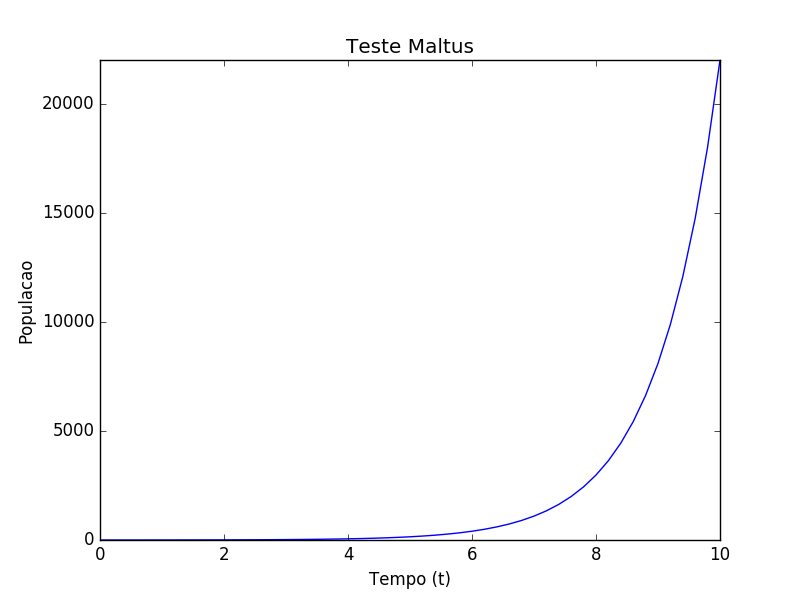
\includegraphics[width=10cm,height=6cm]{resultsCodigos/testeMaltus.png}
                \caption{Resolução numérica do problema \ref{eq:exMalthus}}
                \label{fig:Malthus}
            \end{figure}
            Como podemos ver, a resolução numérica condiz com a solução analítica exponencial.
    
        \subsection{Equações de Lotka-Volterra}
        
            \subsubsection{Definição}
            
        		As equações de Lotka-Volterra foram propostas pelo matemático Vito Volterra e pelo biofísico Alfred J. Lotka no ano de 1925. Elas são um par de equações diferenciais não-lineares e de primeira ordem.
        		 
        		As equações de Lotka-Volterra são mais utilizadas em quadros biológicos envolvendo presas e predadores (como lobos e ovelhas ou golfinhos e peixes), sendo a população das presas considerada a única fonte de alimento para a população de predadores e que não há competição entre os predadores. 
        		
        		Como descrevem um quadro simples, essas equações, em sua definição, não proporcionam uma análise muito próxima da realidade, mas o entendimento sobre elas possibilita o entendimento de situações mais complexas.
		
	        \subsubsection{Principais Situações Descritas pelas Equações}
        		
        		Por suas relações diretas com o contexto de presa-predador, as equações de Lotka-Volterra podem descrever as seguintes situações
		
        		\begin{itemize}
        			\item Extinção de predadores;
        			\item Extinção de presas;
        			\item Existência de predadores e presas ao mesmo tempo;
        			\item Geral.
        		\end{itemize} 
	
        		Cada uma dessas situações para as equações será demonstrada a seguir, considerando $x$ como o número de indivíduos para a população de presas, $y$ para o número de indivíduos da população de predadores e $t$ para o tempo.
		
		    \subsubsection{Caso 01: Extinção de Predadores}
    			
    			Caso $y = 0$ (população de predadores extinta), a população de presas cresce proporcionalmente à população atual, o que é representado por $k$
    			
    				\[y = 0\]
    				
    				\[\frac{dx}{dt} = kx\ \text{, }\qquad k > 0\]
				
		    \subsubsection{Caso 02: Extinção de Presas}
			
    			Caso $x = 0$, ou seja, a população de presas seja extinta, a população de predadores deve se extinguir também, visto que as presas citadas no problema são sua única fonte de alimento. Esse decrescimento na população de predadores se dá proporcionalmente à população atual, sendo tal proporção representada por $r$
    			
    				\[x = 0\]
    				
    				\[\frac{dx}{dt} = - ry \text{, }\qquad r > 0\]
				
		    \subsubsection{Caso 03: Existência de Predadores e Presas ao Mesmo Tempo}
		    
    			Diz-se que as situações em que presa e predador se encontram levam à morte de uma presa e as ocorrências de tais situações são proporcionais ao produtos das populações de presas e predadores. Essa situação é modelada utilizando-se duas constantes de proporcionalidade: $a$ para a taxa de predação e $b$ para a conversão de presa para predador. Logo:
    			
    			\begin{itemize}
    				\item População de presas sofre queda: $-axy$
    				\item População de predadores aumenta: $bxy$
    			\end{itemize}
		
		    \subsubsection{Caso geral}
		    
    			Considerando todos os três casos acima em conjunto, tem-se:
    			
    				\[\frac{dx}{dt} = x (k - a y)\]
    				
    				\[\frac{dy}{dt} = y (r x - b)\]
    			onde $k, a, b \text{ e }r$ relacionam as duas populações.
			
        	\subsubsection{A Relação Entre as Equações de Caso Geral e sua Solução Geral}
	
        		Relacionando ambas as equações de caso geral, encontra-se
        		
        			\[\frac{dy}{dx} = \frac{y (r x - b)}{x (k - a y)}\]
        		cuja solução geral, a partir de integração, é
        		
        			\[k ln(y) - a(y) + C = -b ln(x) + b(x) + D\]
        		sendo C e D constantes de integração \cite{wiki:eqLotkaVolterra}.
        		
        	\subsubsection{Implementação}
        	
        	    O código a seguir propõe uma resolução para um problema de equações de Lotka-Volterra do livro Cálculo, vol. 2, de James Stewart \cite{stewart}. Nesse exemplo, temos que as equações regem as populações de presas e predadores tendo-se
        	    \begin{align*}
        	        k &= 2,0\\
        	        a &= 0,01\\
        	        r &= 0,5\\
        	        b &= 0,0001
        	    \end{align*}
        	    sendo sua condição inicial $t = 0,0$ com 2000 presas e 35 predadores.
        	    
        	    Espera-se que os resultados exibam oscilações entre as populações de presas e predadores. A medida que a população predatória cresce, a de presas deve cair, levando também a predatória a queda, o que fará a de presas subir. Isso deve se dar em ciclos.
        	    
        	    \lstinputlisting[caption=Problema envolvendo as equações de Lotka-Volterra \cite{stewart}, label=LK,firstline=45]{Codigos/testePresaPredador.py}
        	    
        	    \begin{figure}[H]
        	        \centering 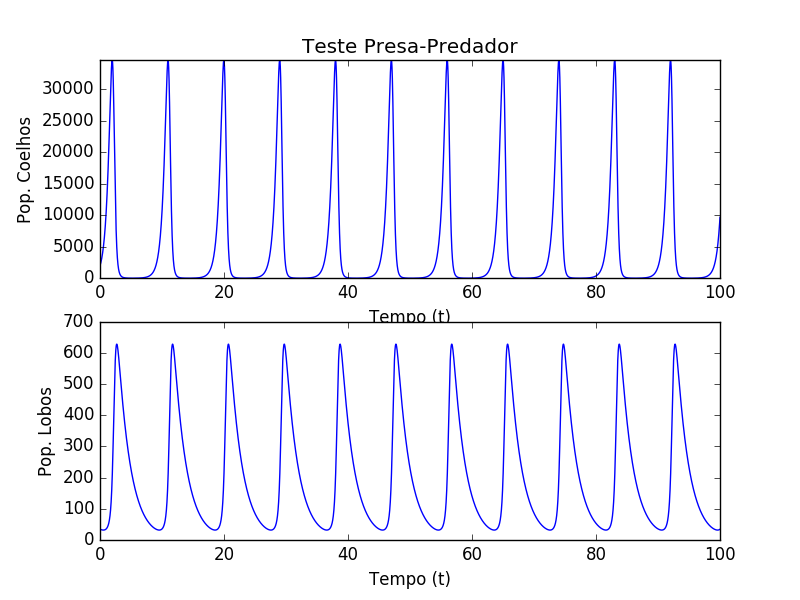
\includegraphics[scale=.8]{resultsCodigos/testePresaPredador.png}
        	        \caption{Resultado do código \ref{LK}}
        	        \label{fig:testPresaPredador}
        	    \end{figure}
        	    
        	    A Figura \ref{fig:testPresaPredador} ilustra, quantitativamente, as populações de joaninhas (predadores) e pulgões (presas) ao longo do tempo $t$. Podemos perceber que logo após a população de presas atingir seus picos, a população de predadores cresce e aplaca as presas, cuja população quase se anula. Com essa rápida queda, a população de predadores tende a decrescer também. Esse processo se repete ao longo do tempo.
        	    
        	    Nesse tipo de problema, as populações de presas e predadores podem sofrer influência de fatores externos também, como o clima. Sendo $\omega$ a frequência da interferência do clima sobre a população de presas, $\alpha$ a amplitude dessa interferência e $\beta$ a média dessa população ao longo do tempo, podemos modelar a influência $K$ do clima sobre a população de presas ao longo do tempo pela equação
        	    \begin{equation}
        	        K(t) = k(1 + \alpha\sin{\omega t} + \beta)
        	    \end{equation}
        	    cujo código em Python se dá por 
        	    
        	    \lstinputlisting[caption=Definição da influência do clima sobre a população de presas ao longo do tempo]{Codigos/influenciaClima.py}
        	    
        	    dentro do método \textit{evaluate} do Código \ref{LK}
        	    
        	    Para esse caso de influência pelo clima obtemos um resultado como da Figura \ref{fig:LCK}. Nele, percebemos que as altas da população de presas se dão próximas à média da variação climática. Crescendo a população de presas, começa a crescer a população predatória, que causa um decrescimento drástico na primeira. Isso leva a população de predadores a decrescer também.
        	    
        	    \begin{figure}[H]
        	        \centering
        	        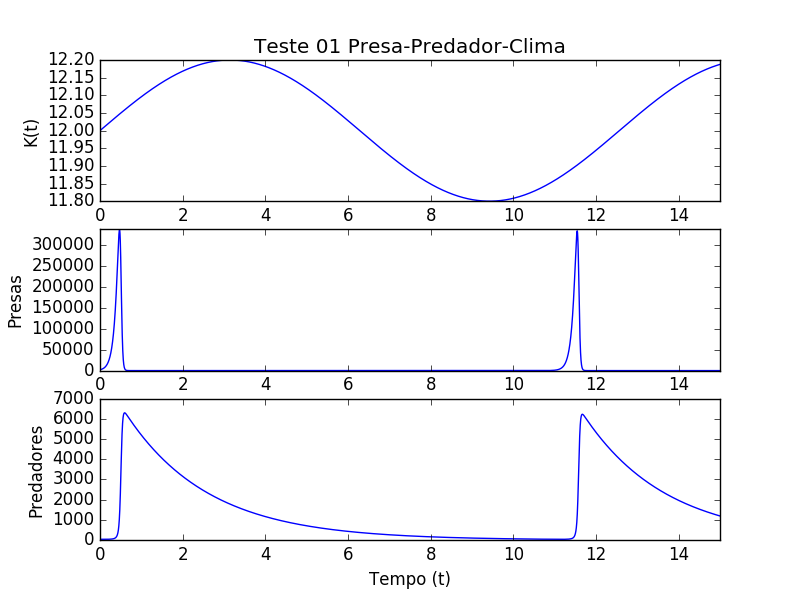
\includegraphics[scale=.6]{resultsCodigos/testePresaPredadorClima01ParaTmax100.png}
        	        \caption{Relação de presas e predatores agora influenciada pelo clima}
        	        \label{fig:LCK}
        	    \end{figure}
    
        \subsection{Sistema Massa-Mola}
        
            Seja um corpo de massa $m$ conectado a uma mola de constante elástica $k$ como na Figura \ref{fig:massaMola}. Esse conjunto é nomeado \textbf{Sistema Massa-Mola}.  
            Os experimentos envolvendo este sistema, em geral, consistem em tirar o conjunto de seu repouso e iniciar sua oscilação, medindo-se então as posições e velocidades do corpo durante as oscilações.
            \begin{figure}[H]
                \centering
                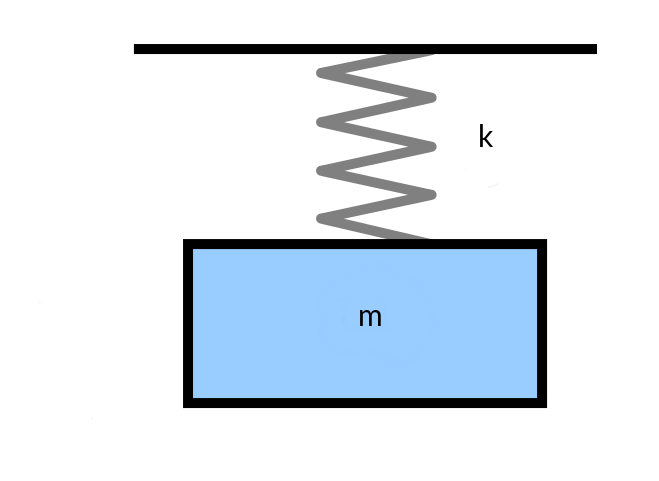
\includegraphics[scale=.25]{imagens/Mass_spring.png}
                \caption{Sistema massa-mola}
                \label{fig:massaMola}
            \end{figure}
            
            O sistema vertical possui três forças agindo sobre ele: a força peso, que podemos nomear por $P$, apontando para baixo, a força elástica da mola, que podemos nomear por $F_e$ e a força de resistência, que nomeamos por $F_r$. $F_e$ última aponta para a direção contrária ao movimento da massa. Essas forças podem ser descritas pelas seguintes equações
            \begin{align}
                P &= mg\\
                F_e &= -ky(t)\\
                F_r &= \gamma y'(t)
            \end{align}
            sendo $g$ a aceleração da gravidade, $y(t)$ o deslocamento feito na mola, $\gamma$ a constante de amortecimento (resistência do ar) e $y'(t)$ a velocidade das oscilações na mola.
            
            Pode haver ainda uma quarta força atuando sobre o sistema: a força externa representada por $F_{ext}$. Essa pode representar, por exemplo, um pistão conectado à mola, que fica gerando outras oscilações no sistema (como veremos na próxima subsubseção) ou, simplesmente, a força gravitacional, como escolhemos para este caso.
            
            Se adotarmos o sistema cartesiano como referencial (termos positivos apontam para cima ou direita, termos negativos apontam para baixo ou esquerda) temos que, pela segunda Lei de Newton
            \begin{align}
                \label{Newton2}
                F &= ma\\
                \intertext{escrevemos a aceleração na forma de derivada}
                F &= my''(t)\\
                \intertext{definimos a força resultante ($F = my''(t)$) como o somatório das forças atuantes sobre o sistema, considerando o sentido das mesmas}
                my''(t) &= F_e + F_r - P\\
                \intertext{substituímos cada força atuante por suas fórmulas}
                \label{eqDifOsc}
                my''(t) &= -ky(t) + \gamma y'(t) - mg\\
                \intertext{isolamos a força externa no lado direito da equação}
                my''(t) - \gamma y'(t) + ky(t) &= -mg
            \end{align}
            essa última equação, satisfeita por $y(t)$ descreve o movimento da massa durante as oscilações do sistema. Nesse tipo de equação, que descreve um comportamento oscilatório, o termo direito representa a força externa $F_{ext}$ que age sobre o sistema. Nesse caso, podemos perceber que $F_{ext}$ é a força gravitacional e que seu sinal negativo indica que ela está apontando para baixo.
            
            O coeficiente $\gamma$ que multiplica $y'(t)$ representa o amortecimento do sistema massa-mola. Empiricamente, o amortecimento pode se dar por um líquido colocado abaixo da massa ou pelo atrito da massa com o ar, por exemplo. O sistema também pode ser considerado sem amortecimento ($\gamma = 0$), o que significa que ele oscilará permanentemente. Mais detalhes sobre o amortecimento desses sistemas podem ser encontrados em \cite{boyce9, regiIntro}.
            
            A solução analítica geral desse sistema é 
            \begin{equation}
                u(t) = c_1\cos{\omega t} + c_2\sin{\omega t}
            \end{equation}
            na qual, $c_1$ e $c_2$ são constantes e $\omega_0$ é a frequência natural dada por $\sqrt{\dfrac{k}{m}}$ do sistema \cite{regiIntro}.
            
            O exemplo a seguir resolve um sistema massa-mola amortecido descrito por 
            \begin{equation*}
                s'' + 0,125s' + s = 0
            \end{equation*}
            com condições iniciais $t = 0.0$, $V_0 = 0.0$ e $P_0 = 2.0$, sendo que $V_0$ e $P_0$ representam, respectivamente, a velocidade e a posição inicial da massa no sistema.
            \lstinputlisting[firstline=45,caption=Código da resolução numérica de um problema envolvendo um sistema massa-mola amortecido]{Codigos/testeMassaMola.py}
            cujo resultado é exibido na figura \ref{fig:MMamortecido}
            \begin{figure}[H]
                \centering
                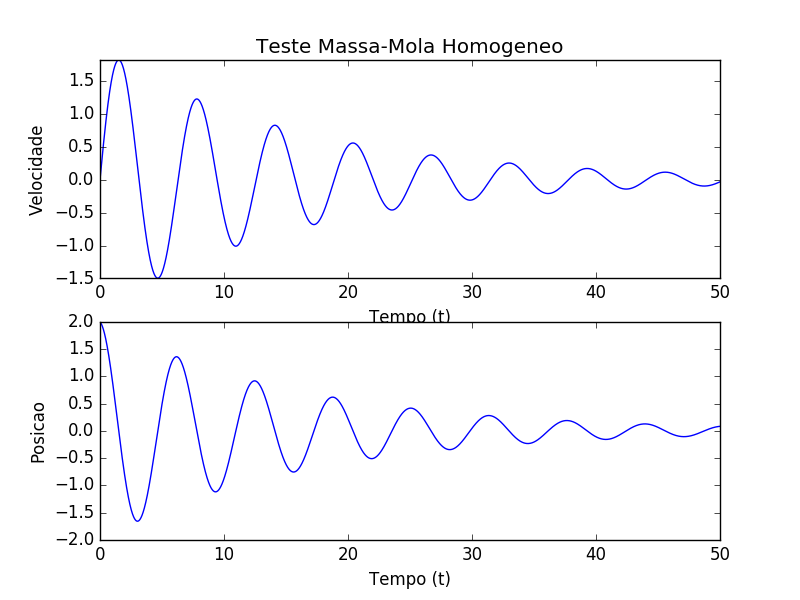
\includegraphics[scale=.54]{imagens/testeMassaMola.png}
                \caption{Gráficos da posição e da velocidade da massa do sistema ao longo do tempo}
                \label{fig:MMamortecido}
            \end{figure}
            
            No primeiro gráfico da Figura \ref{fig:MMamortecido} vemos o gráfico da velocidade da massa em cada instante de tempo.
            Podemos perceber o efeito do amortecimento sobre o sistema pela diminuição da amplitude do movimento e da velocidade dele ao longo do tempo.
            
            \subsubsection{Sistema Massa-Mola Forçado}
    
                Suponha que a força externa $F_{ext}$, que em (\ref{eqDifOsc}) era $-mg$ dependesse do tempo $t$ e fosse periódica, como um pistão que forçasse a mola de um lado para o outro. Teríamos então um \textbf{Sistema Massa-Mola Forçado}, como na Figura \ref{fig:forcedMMS}, no qual $F_{ext} = F_0\cos{\omega t}$, sendo $F_0$ é amplitude da força periódica e $\omega$ é a frequência dela. Nesse sistema ocorre um movimento chamado \textbf{batimento}, que é uma oscilação com uma frequência cuja amplitude também oscila \cite{regiIntro}.
                
                \begin{figure}[H]
                    \centering
                    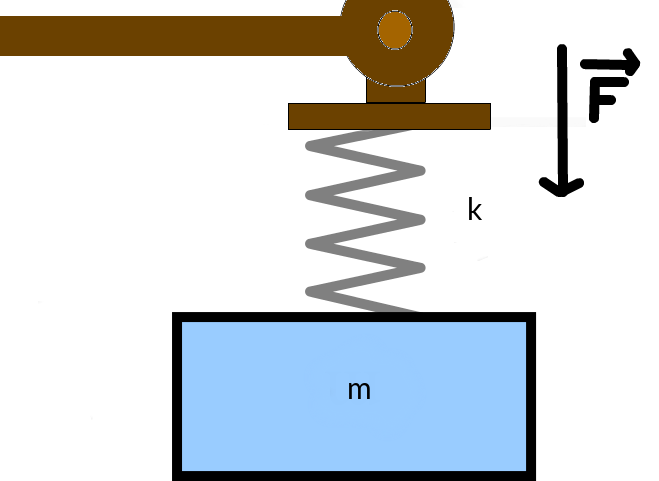
\includegraphics[scale=.3]{imagens/ForcedMass_spring.png}
                    \caption{Imagem meramente ilustrativa de um sistema massa-mola forçado}
                    \label{fig:forcedMMS}
                \end{figure}
                
                A solução analítica geral desse caso se dá por
                \begin{align}
                    u(t) &= c_1\cos{\omega_0t} + c_2\sin{\omega_0t} + u_p(t) \\\text{ com		}
                    \label{solPart}
                    u_p(t) &= t^s[A\cos{\omega t} + B\sin{\omega t}]
                \end{align}
                sendo $c_1$ e $c_2$ constantes da solução geral e $\omega_0$ a frequência natural do sistema. O termo $u_p(t)$ é a solução particular (também chamada solução transiente \cite{boyce9}) do problema na qual $s$ é ``o menor inteiro não negativo que garanta que nenhuma parcela de $u_p(t)$ seja solução da equação homogênea correspondente [...]'' \cite{regiIntro} e $A$ e $B$ são coeficientes da solução que podem ser determinados pelo método de coeficientes a determinar, como pode ser visto em \cite{regiIntro}.
                
                O código a seguir resolve, matematica e numericamente, o mesmo sistema massa-mola apresentado no exemplo anterior, porém agora com uma força externa agindo sobre o mesmo. A força externa $F_{ext}$ é descrita por
                \begin{equation*}
                    F_{ext} = \cos{\omega_0t}
                \end{equation*}
                \lstinputlisting[firstline=57,caption=Código da resolução numérica de um problema envolvendo um sistema massa-mola forçado]{Codigos/testeMassaMolaForcado.py}
                cujo resultado é exibido na Figura \ref{fig:MMforcado}
                \begin{figure}[H]
                    \centering 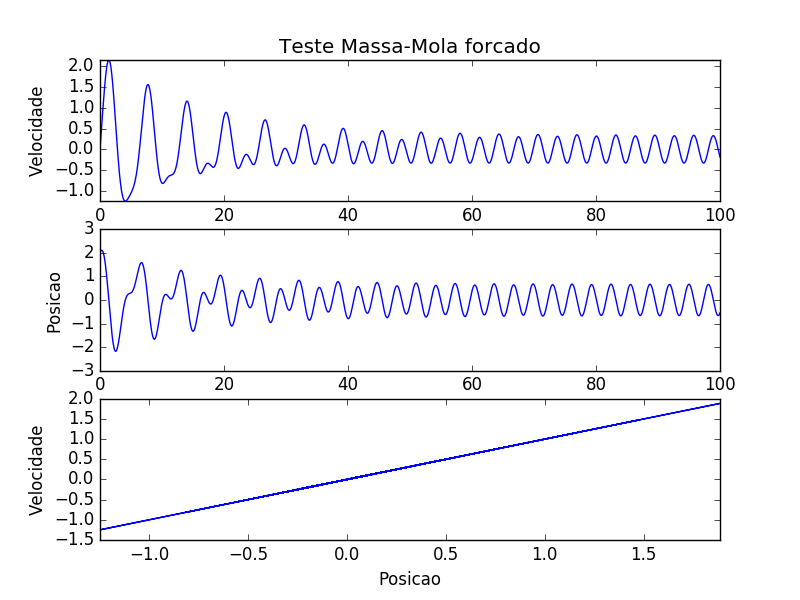
\includegraphics[scale=.54]{imagens/testeMassaMolaForcado.png}
                    \caption{Gráficos da posição e da velocidade da massa do sistema ao longo do tempo, seguido de um gráfico da velocidade pela posição}
                    \label{fig:MMforcado}
                \end{figure}
                
                O primeiro gráfico descreve a velocidade $v$ ao longo do tempo $t$ e o segundo descreve a posição $y$ da massa ao longo de $t$ também. Podemos perceber a ação da solução transiente até cerca de 50 unidades de tempo em ambos os gráficos, sendo que permanece depois apenas a solução geral (também chamada solução estado estacionário - \cite{boyce9}).
                
                O terceiro gráfico descreve a velocidade $v(t)$ em função da posição $y(t)$ da massa. O sinal da velocidade indica o sentido dela.
    
    \chapter{Ondulatória}

    \label{cap:ond}

	\section{Definição}
		Ondas são pertubações que se propagam através do espaço e/ou meio material, transportando energia, por meio de oscilações periódicas e com velocidade constante \cite{moises}. 
		Elas estão continuamente presentes no cotidiano humano, como nas ondas sonoras, micro-ondas, as ondas marítimas e a própria luz.
		
		As ondas possuem propriedades físicas, características e podem ser classificadas quanto a sua natureza, direção de oscilação e de propagação.
		
	\section{Classificações Quanto à Natureza}
		Com relação à natureza das ondas, elas podem ser classificadas em três tipos, principalmente \cite{halliday}
		\begin{enumerate}
			\item\textbf{Mecânicas: }são as ondas que se movimentam apenas em meio material e obedecem às Leis de Newton. Alguns exemplos dessas ondas são as sonoras, marítimas e sísmicas.

			\item\textbf{Eletromagnéticas: }ondas criadas pela interação entre um campo elétrico e um campo magnético. Ao contrário das ondas mecânicas, essas não necessitam de meio material para a sua propagação, podendo se movimentar até mesmo no vácuo (no qual todas as ondas eletromagnéticas alcançam a velocidade da luz). Alguns exemplos dessas ondas são a própria luz, as ondas de rádio e as ondas emitidas por aparelhos micro-ondas.
			
			\item\textbf{Materiais: }estão relacionadas aos elementos mais básicos da matéria, como prótons e elétrons. Por causa disso, são mais estudadas em laboratórios.
		\end{enumerate}
		
	\section{Classificações Quanto à Direção de Oscilação}
		Com relação à direção que as ondas oscilam (principalmente as mecânicas), elas podem ser classificadas em dois tipos,
		\begin{enumerate}
			\item\textbf{Transversais: }são as ondas nas quais os elementos do meio no qual ela propaga	se movimentam perpendicularmente a sua direção de propagação. Por exemplo, se um indivíduo amarrar a ponta de um barbante longo em um objeto fixo e sacudir a outra ponta para cima e para baixo rapidamente, uma onda será transmitida ao longo do barbante em formato de pulso. As partículas da corda subirão e descerão, movimentando-se perpendicularmente ao movimento da onda, que segue a estrutura do barbante.
			
			\item\textbf{Longitudinais: }são as ondas nas quais os elementos do meio em que ela se propaga se movimentam no mesmo sentido que a onda se propaga. Um exemplo desse caso são as ondas sonoras. Elas são transmitidas por pulsos longitudinais no ar. Por exemplo, em um tubo com ar, se for colocado um êmbolo em uma de suas extremidades e este for movimentado bruscamente para frente e, em seguida, para trás, será gerada uma onda sonora e na estrutura do meio em que ela se propaga (o próprio ar) seria possível perceber que o movimento das moléculas se dá no sentido do pulso da onda sonora \cite{halliday}. 
			
		\end{enumerate}
	
	\section{Classificações Quanto à Direção de Propagação}
		Com relação à direção que as ondas se propagam (o comportamento das ondas em diferentes dimensões), elas podem ser classificadas em três tipos \cite{wiki:onda}
		\begin{enumerate}
			\item\textbf{Unidimensionais: }são as que se propagam apenas em uma direção, como pulsos em cordas.
			
			\item\textbf{Bidimensionais: }são as que se propagam em duas direções, em um plano, como as vibrações em uma folha de papel chacoalhada ou as vibrações em um espelho d'água após alguém atiram uma pedra sobre ele.
			
			\item\textbf{Tridimensionais: }são as que se propagam no espaço, em três direções, como as ondas sonoras no ar.
		\end{enumerate}
	
	\section{Características Gerais das Ondas}
		Em decorrência do fato de que as ondas oscilam periodicamente, algumas características gerais do fenômeno podem ser estudadas sobre este fato \cite{halliday}
		\begin{itemize}
			\item\textbf{Comprimento: }intervalo no espaço, paralelo à direção da propagação da onda, em que se inicia e termina uma onda (oscilação completa), se iniciando outra logo em seguida; 
			
			\item\textbf{Amplitude: }deslocamento máximo e mínimo efetuado por um elemento do meio em que a onda se propaga quando a onda passa por ele. Por exemplo, a altura máxima e mínima alcançada por uma partícula de uma corda na qual foi efetuado um pulso quando o pulso passa pela partícula; 
			
			\item\textbf{Período: }espaço de tempo necessário para a realização de uma oscilação completa; 
			
			\item\textbf{Frequência: }número de oscilações completas por unidade de tempo (segundos no Sistema Internacional de Unidades); 
			\item\textbf{Fase: }corresponde ao intervalo no espaço em que um elemento do meio em que a onda se propaga alcança suas amplitudes máxima e mínima, como uma partícula de uma corda alcançando a crista e o vale de um pulso emitido na mesma corda (ou seja, realizando uma oscilação completa).
		\end{itemize}
	
	\section{Propriedades Físicas das Ondas}
		Por ser um fenômeno físico, é de se esperar que a ondulatória obedeça as leis da Física, o que lhe atribui algumas propriedades físicas
		\begin{itemize}
			\item\textbf{Superposição: }No estudo de ondas, há também a questão da superposicão das ondas lineares, sendo que quando ondas se superpõem elas se somam algebricamente, gerando uma onda resultante ou uma onda total, sem se afetar mutuamente. Essa propriedade é consequência direta do princípio da superposição, que afirma que a ocorrência simultânea de efeitos individuais leva à formação de um efeito total formado pela soma dos individuais. Isso ocorre por exemplo, em lagos nos quais as ondas provocadas por embarcações se superpõem continuamente. Isso ocorre também em uma rua com tráfego intenso, na qual o barulho dos automóveis se superpõem uns aos outros, chegando ao mesmo tempo aos ouvidos das pessoas que ali estão \cite{halliday}; 
			
			\item\textbf{Interferência: }ocorre como consequência da superposição de ondas e depende da fase relativa das duas ondas. Ou seja, se elas estão alinhadas (em fase) e com amplitude igual, seu deslocamento conjunto ocorre em dobro. Se elas não estão alinhadas (fora de fase) e, novamente, com amplitude igual, seu deslocamento é nulo, pois elas se cancelam. Em consequência desse fenômeno, se duas ondas de mesma amplitude e comprimento se movimentarem em um meio, uma contra a outra, a onda resultante será chamada estacionária, pois não se move para nenhum lado e possui pontos que são fixos \cite{halliday}; 
			
			\item\textbf{Reflexão: }quando uma onda está se propagando por um meio e se depara com outro meio de características estruturais diferentes, ela sofre interferência em si mesma e é refletida. Por exemplo, se um barbante está preso a um ponto imóvel e um pulso é emitido nele, quando o mesmo chegar ao ponto fixo, a terceira Lei de Newton agirá, criando um pulso de mesma amplitude, comprimento mas sentido e posição contrários. Já se o ponto em que o barbante estiver preso for móvel, a reflexão ocorrerá da mesma forma, mas a posição do pulso refletido será a mesma do pulso original \cite{halliday}; 
			
			\item\textbf{Refração: }quando a onda entra em contato com outro meio material, sua direção e velocidade variam, mas sua frequência se mantem \cite{seth}; 
			
			\item\textbf{Difração: }quando ocorre o espalhamento de ondas após uma onda entrar em contato com uma fenda com tamanho equivalente ao seu comprimento \cite{seth};
			
			\item\textbf{Dispersão: }quando uma onda se separa em outras de diferentes frequências \cite{seth}; 
			
			\item\textbf{Vibração: }ondas produzidas através de vibrações de objetos, como cordas de violão ou tubos de flauta \cite{seth}; 
			
			\item\textbf{Polarização: }como já vimos anteriormente, em uma onda transversal as oscilações são em alguma direção perpendicular à direção de propagação da onda. Dessa forma, uma onda pode oscilar para baixo, para a direita, para a esquerda, etc\dots. A fixação da direção de oscilação de uma onda, fazendo com que ele oscile apenas em uma direção só, é chamada polarização \cite{wiki:polarization}.
			
			\item\textbf{Ressonância: }suponha, por exemplo, fossem criados vários pulsos indo para a direita em um barbante e este estiver preso em sua extremidade direita. Quando o primeiro pulso alcançasse a extremidade e fosse refletido, começaria a voltar pelo barbante e, pelo princípio da superposição, geraria interferência no contato com os outros pontos. Esse pulso em questão (e os demais por consequência) chegaria à extremidade esquerda e seria refletido e, em seguida, novas interferências seriam geradas. Em certas frequências, a interferência entre os pulsos gera ondas estacionárias (que permanecem no mesmo lugar, sem locomoção) por ressonância \cite{halliday}.  
			
		\end{itemize}
	
	\section{As Ondas Transportam Energia, Não Matéria}
		É necessário saber e entender que uma onda não transporta matéria, somente energia. Quando uma ginasta olímpica cria um pulso em uma fita, por exemplo, fornece-se energia para o movimento da fita, que é transportada ao longo dela. Essa energia se apresenta em forma de energia cinética e energia potencial elástica. 
				
		É possível se observar a energia cinética através do movimento oscilatório de cada parte da fita, quando cada partícula vai até a crista e desce até o vale. Já a energia potencial elástica se deve ao fato de que cada parte da fita é esticada e comprimida (como uma mola) enquanto a onda passa por ela. A energia é transportada ao longo da fita pelo trabalho das forças de tensão que ligam as partes da fita.
	
	\section{A Equação Geral de Deslocamento da Onda}
	
		Sabe-se que uma onda cujos pontos não se locomovem espacialmente é chamada onda estacionária \cite{wiki:stateWave}. Já uma onda que se locomove enquanto se propaga é chamada senoidal. Isso pode ser justificado pela equação geral de deslocamento de uma onda
		
		\[y(x,t)=y_{m}\sin(kx-\omega t)\]
		
		na qual, $t$ representa o tempo, $y_{m}$ representa o deslocamento paralelo ao eixo $y$ dos elementos do meio onde a onda se propaga (amplitude), $x$ é a posição do referido elemento, $\omega$ representa a frequência angular e o elemento $k$ representa o número de onda.
		
		Nessa equação, percebe-se a existência de uma função seno: $\sin(kx-\omega t)$, que é responsável por expressar matematicamente as oscilações das ondas em sua locomoção e propagação, já que é uma função periódica, assim como a função cosseno. Fato observável na representação gráfica das funções seno e cosseno a seguir, juntamente com o código utilizado para gerá-las
		
		\begin{figure}[H]
			\centering
			\begin{minipage}{.5\textwidth}
				\centering
				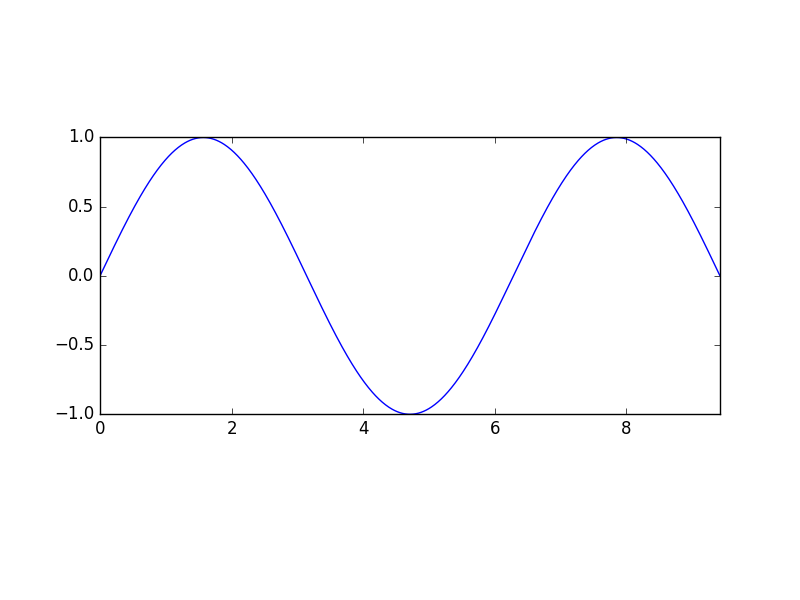
\includegraphics[scale=.35]{resultsCodigos/seno3}
				\captionof{figure}{Gráfico da função $y(x) = \sin(x)$}
			\end{minipage}%
			\begin{minipage}{.5\textwidth}
				\centering
				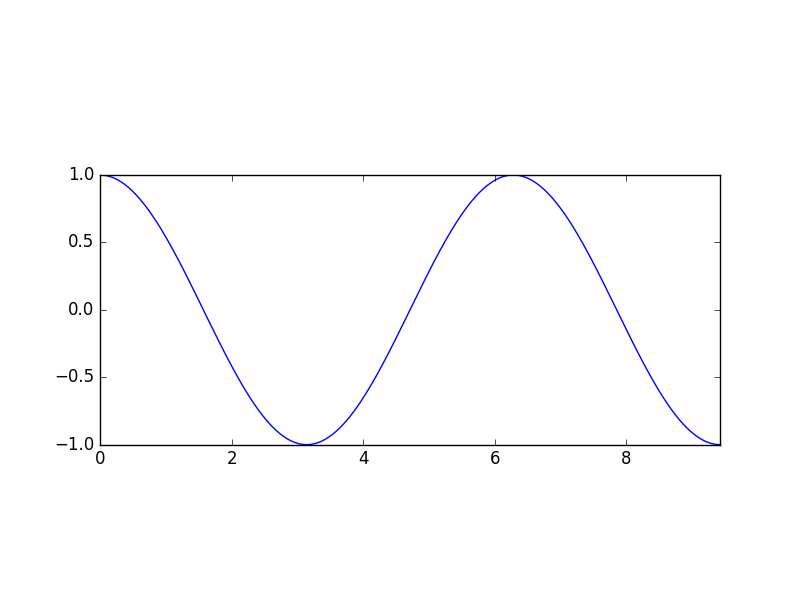
\includegraphics[scale=.35]{resultsCodigos/cosseno}
				\captionof{figure}{Gráfico da função $y(x) = \cos(x)$}
			\end{minipage}
		\end{figure}
		
		Dessa forma, pode-se entender o motivo do nome senoidal.
		
		\lstset{language=Python}
		\begin{lstlisting}
#Codigo para plotagem do seno

import numpy as np
import matplotlib.pyplot as plt

pi = 3.14159265359
xvals = np.arange(0, 3*pi, 0.01)
yvals = np.sin(xvals)
plt.plot(xvals, yvals)
plt.axis([0, 3*pi, -1, 1])
plt.show()
		\end{lstlisting}
		
		\begin{lstlisting}
#Codigo para plotagem do cosseno

import numpy as np
import matplotlib.pyplot as plt

pi = 3.14159265359
xvals = np.arange(0, 3*pi, 0.01)
yvals = np.cos(xvals)
plt.plot(xvals, yvals)
plt.axis([0, 3*pi, -1, 1])
plt.show()
		\end{lstlisting}
		
	\section{A Equação Geral da Onda}
		O comportamento das ondas pode ser estudado através da equação geral da onda
		
		\begin{equation}
		    \frac{\partial^2 u}{\partial t^2} = \frac{1}{v}\frac{\partial^2 u}{\partial x^2}
		\end{equation}
		na qual, $v$ representa a velocidade de propagação da onda e $t$ representa o tempo. Essa equação foi obtida por meio da aplicação da segunda lei de Newton ao movimento dos elementos do meio em que a onda se propaga, como os elementos de uma fita, por exemplo. Essa equação é uma equação diferencial geral parcial (a ser estudada mais a fundo no capítulo \ref{cap:EDPs}), o que indica que existem taxas que se relacionam no fenômeno.
	
	\section{Algumas Aplicações do Estudo de Ondas}
		Como dito anteriormente, o estudo do fenômeno físico das ondas possibilita um melhor bem-estar para a humanidade. Ele pode ser utilizado, por exemplo, nas áreas:
		\begin{itemize}
			\item\textbf{Acústica: }o estudo apropriado das ondas sonoras facilita o alcance do som de uma orquestra até a sua plateia, por exemplo, contribuindo para as Artes e Cultura;
			
			\item\textbf{Sísmica: }o estudo sobre as ondas sísmicas podem facilitar a previsão de terremotos e a evolução da tecnologia de prédios resistentes a tremores de alta intensidade;
			
			\item\textbf{Estruturas: }pontes usadas em grandes estradas, por exemplo, costumam estar em contato constante com ondas marítimas ou fluviais, além do próprio vento. Se os cálculos dos engenheiros responsáveis pela construção das mesmas não assegurar a estabilidade da ponte, a mesma pode ruir pelo fenômeno da ressonância ou pelo impacto constante das ondas.
			
		\end{itemize}


    
    \chapter{Equações Diferenciais Parciais e a Equação da Onda}

    \label{cap:EDPs}

    \section{Definição de uma Equação Diferencial Parcial e Alguns Exemplos}
    
        \label{EDPdef}
    
        Uma equação diferencial parcial (EDP) é baseada numa função como
        \begin{equation}
            \label{defMatEDP}
            f(x_1, x_2, ..., y, \dfrac{dy}{dx_1}, ..., \dfrac{dy}{dx_n}, 
            \dfrac{d^2y}{dx_1dx_1}, ...,\dfrac{d^2y}{dx_1dx_n}, ...) = c
        \end{equation}
        na qual $c$ é uma constante, ou seja, em uma função de $y$ e suas derivadas parciais.
        Por meio dessa definição podemos perceber, assim como já tinha sido dito na seção \ref{defEDO}, 
        que uma EDP possui mais de uma variável independente. Uma EDP baseada numa função como \ref{defMatEDP}, mas com $c = 0$, é dita equação diferencial parcial linear \cite{wiki:EDP}. Por exemplo, uma EDP linear de segunda ordem seria na forma \cite{EDPWolfram}
        \begin{equation}
            \label{EDPlin2}
            Ay_{x_1x_1} + By_{x_1x_2} + Cy_{x_2x_2} + Dy_{x_1} + Ey_{x_2} + F = 0
        \end{equation}
        
        Alguns exemplos de EDP's são: 
        \begin{itemize}
            \item $u_t = a^2u_{xx}$, a equação unidimensional do calor (sendo $u_t = a^2(u_{xx}+u_{yy})$ a sua versão bidimensional) que determina a distribuição do calor através da(s) dimensão(ões) de um corpo ao longo do tempo;
            \item $u_{xx} + u_{yy} = 0$, a equação bidimensional de Laplace (sendo $u_{xx} + u_{yy} + u_{zz}+ = 0$ sua versão tridimensional), que serve de modelo para as funções potenciais gravitacionais e elétricas, por exemplo \cite{wiki:LaplaceEq};
            \item $u_{tt} = a^2u_{xx}$, a equação unidimensional da onda (sendo sua versão bidimensional $u_{tt} = a^2(u_{xx} + u_{yy})$ e a tridimensional, $u_{tt} = a^2(u_{xx} + u_{yy} + u_{zz})$), que descreve o comportamento das ondas das mais variadas naturezas (e que é peça-chave desse projeto) \cite{EDPSodrenotas}.
        \end{itemize}
        
            \subsection{Tipos de Equações Diferencias Parciais}
        
                \subsubsection{Equações Diferenciais Parciais Elípticas}
                
                    Considerando uma equação como (\ref{EDPlin2}), ela é dita elíptica quando $B^2 - AC < 0$ \cite{wiki:EDP}. Podemos perceber que equações como a de Laplace, citada na seção anterior, que são elípticas, seguem o formado da equação da cônica elipse
                    \begin{equation*}
                        \frac{x^2}{a^2} + \frac{y^2}{b^2} = c^2
                    \end{equation*}
                    ou da quádrica elipsóide,
                    \begin{equation*}
                        \frac{x^2}{a^2} + \frac{y^2}{b^2} + \frac{z^2}{c^2}= d^2
                    \end{equation*}
                    dependendo do número de dimensões consideradas.
                
                \subsubsection{Equações Diferenciais Parciais Parabólicas}
                
                    Ainda considerando uma equação como (\ref{EDPlin2}), caso $B^2 - AC = 0$, essa equação é do tipo parabólica \cite{wiki:EDP}. Podemos ver que equações como a do calor, apresentada na seção \ref{EDPdef}, tem o mesmo formato que a cônica parábola \cite{wiki:parabola}
                    \begin{equation*}
                        y^2 = 4px
                    \end{equation*}
                    ou da quádrica parabolóide,
                    \begin{equation*}
                        \frac{x^2}{a^2} + \frac{y^2}{b^2} = \frac{z}{c}
                    \end{equation*}
                    dependendo do número de dimensões consideradas \cite{wiki:paraboloide}.
                
                \subsubsection{Equações Diferenciais Parciais Hiperbólicas}
        
                    Mais uma vez considerando a equação (\ref{EDPlin2}), se $B^2 - AC > 0$ então a equação é do tipo hiperbólica, como a equação da onda citada em (\ref{EDPdef}). Assim como as equações anteriores, as EDP's anteriores são similares à equação da cônica hipérbole
                    \begin{equation}
                        \frac{x^2}{a^2} - \frac{y^2}{b^2} = c^2
                    \end{equation}
                    ou da quádrica hiperboloide,
                    \begin{equation*}
                        \frac{x^2}{a^2} + \frac{y^2}{b^2} - \frac{z^2}{c^2} = d^2
                    \end{equation*}
        
    \section{Resolução de Equações Diferenciais Parciais}
        
        As EDP's podem ser resolvidas ou analítica ou 
        numericamente. Dentre os métodos de resolução analítica encontramos:
        \begin{itemize}
            \item separação de variáveis;
            \item método das características;
            \item mudança de variáveis;
        \end{itemize}
        entre outras opções, que podem ser encontradas em \cite{wiki:EDP}.
        
        Contudo, esses métodos nem sempre são suficientes para resolver os problemas 
        que envolvem as EDP's, sendo necessário então recorrer ao métodos numéricos, entre eles os mais comuns
        \begin{itemize}
            \item método das diferenças finitas;
            \item método dos elementos finitos;
            \item método dos volumes finitos \cite{wiki:EDP};
        \end{itemize}
        dos quais usaremos apenas o primeiro mais a frente. Também utilizaremos, por 
        trabalharmos com a equação da onda neste projeto, o método de traçamento de raios.
    
	\section{A Equação da Onda}
	    \subsection{Em uma Dimensão Espacial}
    		A equação da onda é uma equação diferencial parcial hiperbólica que segue o seguinte formato para casos unidimensionais sem fonte de emissão para a onda:
    		\begin{equation}
    			\frac{\partial^2 u}{\partial t^2} = \frac{1}{v}\frac{\partial^2 u}{\partial x^2}
    			\label{eqOnda1Dh}
    		\end{equation}
    		e, para casos onde há fonte de emissão da onda:
    		\begin{equation}	
    			\frac{\partial^2 u}{\partial t^2} = \frac{1}{v}\frac{\partial^2 u}{\partial x^2} + f(x, t)
    			\label{eqOnda1Dnh}	
    		\end{equation}
    		na qual $v$ representa a velocidade de propagação da onda e $f(x, t)$  é uma função que representa a fonte de emissão da onda.
    		Essas equações (ou alguma generalização delas) definem o comportamento de uma onda, seja ela de natureza acústica, aquática, 
    		eletromagnética ou sísmica, por exemplo \cite{boyce9}.
    		
    		Durante a modelagem de um problema físico envolvendo a propagação de ondas é necessário, além, claro, da equação da onda, a definição de condições de fronteira (também conhecidas como condições de contorno) e uma condição inicial. Supondo uma corda de comprimento $L$, fixada nos pontos $x = 0$ e $x = L$, tem-se como condições de fronteira
    		\[u(0, t) = u_{a}\text{, } u(L, t) = u_{b}\]
    		e como condições iniciais
    		\[u(x, 0) = f(x)\text{, } 0\le x\le L\text{ para a posição inicial}\]
    		\[\text{e } u_{t}(x, 0) = g(x)\text{, } 0\le x\le L\text{ para a velocidade inicial}\]
            Se $u_a = u_b = 0$, por exemplo, temos que a onda refletirá nas bordas do domínio considerado.
    
    		A solução $u(x, t)$ da EDP descreve o deslocamento vertical da corda no ponto $x$, em um instante $t$ de tempo \cite{boyce9}.
		
	    \subsection{Em duas Dimensões Espaciais}
	
	        Imagine uma membrana elástica, como uma membrana de tambor ou até mesmo o tímpano que se encontra no nosso ouvido. Nessa membrana, cada ponto $(x, y)$ está ligado ao seus vizinhos de modo que, se a membrana é excitada ela vibra ou de acordo com a equação
	        \begin{equation}
	            \dfrac{\partial^2u}{\partial t^2} = \frac{1}{v}(\dfrac{\partial^2u}{\partial x^2} + \dfrac{\partial^2u}{\partial x^2})
	        \end{equation}
	        ou, se a excitação for realizada por uma fonte, pela equação
	        \begin{equation}
	            \dfrac{\partial^2u}{\partial t^2} = \frac{1}{v}(\dfrac{\partial^2u}{\partial x^2} + \dfrac{\partial^2u}{\partial x^2}) + f(x, y, t)
	        \end{equation}
	        Se tal membrana, ou o meio pelo qual a onda se propaga, for homogêneo, $v$ é constante. Do contrário, $v$ é uma função em $x$ e $y$.
	        
	        A ligação de cada ponto $(x, y)$ aos seus vizinhos, de modo que qualquer excitação na membrana gere oscilações por ela, pode ser imaginada como um sistema massa-mola infinito (ou quase infinito). Para isso, basta que assumamos cada ponto como uma massa infinitesimal $m$ e cada ligação como uma pequena mola de constante elástica $k$. As pequenas molas são os elementos que levam à vibração.
	        
	        Assim como o caso unidimensional, o modelo da propagação de ondas em meios bidimensionais necessita de uma condição inicial (quando a baqueta toca a membrana de um tambor de uma bateria) e de condições de contorno (a membrana tem seu contorno ligado a um suporte). Podemos definir as condições de contorno como \cite{dailedaWE}
	        \begin{align}
	            \label{eq:condContorno}
	            u(0, y, t) = u(a, y, t) = 0,\ \ \ \ \ \ \ \ 0\le x \le a, \ t \ge 0,\\
	            u(x, 0, t) = u(x, b, t) = 0,\ \ \ \ \ \ \ \ 0\le y \le b, \ t \ge 0.
	        \end{align}
	        e as condições iniciais como
	        \begin{align}
	        \label{eq:condIniciais}
	            u(x, y, 0) &= f(x, y),\\
	            u_t(x, y, 0) &= g(x, y)
	        \end{align}
    
    \chapter{O Método de Diferenças Finitas}

    \label{cap:MDF}
    
    O método de diferenças finitas (MDF) vem com o objetivo principal de aproximar derivadas
    de funções, servindo também na resolução de EDO's e EDP's. Essa aproximação se dá discretizando-se o domínio no qual a função será aplicada e combinando valores de uma função (que estejam próximos uns dos outros) através de certas fórmulas,
    usando determinados pesos em conjunto aos valores da função \cite{scholarMDF}.

    \section{Diferenças Finitas}
    
        Uma diferença finita é definida por um quociente de diferenças como
        \begin{equation}
            \label{progFD}
            \dfrac{f(x + \Delta x) - f(x)}{\Delta x}
        \end{equation}
        Pode-se perceber a similaridade da expressão acima com
        \begin{equation}
            \dfrac{f(x_0 + h) - f(x_0)}{h}
        \end{equation}
        que, como sabemos, tende para $f'(x_0)$ quando $h \xrightarrow{} 0$. Então, se fizermos
        $x = x_0$, $\Delta x = h$ e $\Delta x \xrightarrow{} 0$, temos que a equação (\ref{progFD}) é uma 
        aproximação de $f'(x_0)$ e, sendo assim, podemos chamá-la \textbf{diferença finita progressiva} de 
        ordem um (sendo ordem referente à acurácia da fórmula em relação à função analítica) \cite{CalcNumUFGRS}. 
        Por meio disso podemos perceber o motivo pelo qual se utiliza as diferenças finitas para a aproximação de derivadas.
    
    \section{Fórmulas de Diferenças Finitas}
    
        Como vimos na seção anterior, podemos obter uma fórmula para diferenças finitas progressivas de ordem um. Além desse tipo, existem dois outros tipos de fórmulas de diferenças finitas \cite{ChenMDF}
        \begin{itemize}
            \item regressivas, \textit{e. g.}
            \begin{equation}
                \label{regrlFD}
                f'(x_0) \cong \dfrac{f(x_0) - f(x_0 - \Delta x)}{\Delta x}\text{, também de ordem um;}
            \end{equation}
            \item centrais, \textit{e. g.}
            \begin{equation}
                \label{centralFD}
                f'(x_0) \cong \dfrac{f(x_0 + \Delta x) - f(x_0 - \Delta x)}{\Delta x}\text{, ainda de ordem um}
            \end{equation}
        \end{itemize}
        Cada uma delas pode ser a melhor para uma determinada situação.
        
        % Nas fórmulas apresentadas acima, podemos perceber que tanto os coeficientes que multiplicam os valores das funções quanto 
        % os denominadores das fórmulas são constantes. Para cada ordem dessas fórmulas esses valores são diferentes (além de mais pontos poderem ser exigidos)
        
        Para a afirmação a seguir, assuma que $f(x_i + j\Delta x) = u_{i + j}$, sendo $i$ a posição do \textit{array} $u$ em que o MDF está centrado, $j$ um valor inteiro para referenciar um vizinho do centro e que $u_w$ representa $f(x_w)$. Dependendo das derivadas requeridas para o método de diferenças finitas, o número de chamadas à função bem como os coeficientes que as acompanham, além dos denominadores das expressões, serão diferentes. Se representarmos graficamente essas fórmulas, perceberemos que elas possuem formatos específicos que damos o nome de \textit{stencil} (ou estêncil, em português). Por exemplo, as fórmulas de diferenças finitas de ordem dois para a segunda derivada $f''(x)$ em uma dimensão (usadas na aplicação do MDF sobre a equação da onda) são:
        \begin{itemize}
            \item regressivas
            \begin{equation}
                \label{u''Reg}
                \dfrac{u_i - 2u_{i-1} + u_{i-2}}{(\Delta x)^2}\text{;}
            \end{equation}
            \item progressivas
            \begin{equation}
                \label{u''Prog}
                \dfrac{u_{i+2} - 2u_{i+1} + u_i}{(\Delta x)^2}\text{;}
            \end{equation}
            \item centrais
            \begin{equation}
                \label{u''Cent}
                \dfrac{u_{i+1} - 2u_{i} + u_{i-1}}{(\Delta x)^2}\text{ \cite{ChenMDF}.}
            \end{equation}
            
        \end{itemize}
        
        \section{As Diferenças Finitas e as Dimensões}
        
            Se um dado problema envolve uma função $u$, com $n$ variáveis (ou seja, $n$ dimensões), e suas respectivas derivadas, é necessário que o método de diferenças finitas seja aplicado de acordo com as variáveis da função $u$. Ou seja, se para $u$ com uma variável tínhamos a indexação do \textit{array} (o que representa os valores da função) como sendo $u_{i + j}$, como explicado na seção anterior, agora teremos $u_{i_1 + j_1, i_2 + j_2, ..., i_n + j_n}$ como representação para a indexação do \textit{array} $n$-dimensional \cite{notasAulas2017}. 
            
            Nessa representação, $i_1, i_2, ..., i_n$ representam as posições do \textit{array} $u$ e $j_1, j_2, ..., j_n$ representam os deslocamentos dessas posições até seus vizinhos em uma determinada dimensão. A dimensão, por sua vez, é dada pela ordem dos $i$'s na indexação. Para tentar deixar mais claro, podemos dar como exemplo a função $u$ com  \cite{notasAulas2017}
            \begin{itemize}
                \item duas dimensões
                \begin{equation}
                    u(x_i, t_j) \equiv u_{i, j}\text{;} 
                \end{equation}
                \item três dimensões
                \begin{equation}
                    u(x_i, y_j, t_k) \equiv u_{i, j, k}
                \end{equation}
            \end{itemize}
            
        \section{Como o Método é Aplicado?}
        
            A maneira como o método é aplicado pode variar um pouco dependendo da finalidade para o qual ele é utilizado. Contudo, ele segue etapas gerais que enunciaremos e explicaremos aqui.
            
            \subsection{Discretização}
            
                Como sabemos, é impossível que nossos computadores consigam representar um domínio contínuo, visto que, por exemplo, entre dois números naturais existem infinitos números reais. Dessa forma, torna-se necessária a discretização do domínio em que o problema que desejamos resolver está inserido.
                
                Imagine o domínio desse problema (considerando aqui o caso unidimensional para a propagação de ondas) como uma cama retangular de comprimento $a$ e largura $b$. Essa cama representa o espaço-tempo unidimensional para o problema. Sendo assim, temos que a variável que percorre o comprimento da cama seja $x$ e a que percorre a largura seja $t$. Então temos que a cama, contínua, é dado por 
                \begin{align*}
                    0 \leq  &x \leq a\\
                    0 \leq  &t \leq b
                \end{align*}
                
                Agora imagine que precisemos que essa cama elástica seja representada numerica ou computacionalmente. Para tal, dividimos seu comprimento e sua largura em espaços de mesmo tamanho, que podem ser iguais para o comprimento e a largura da cama ou diferentes para cada um desses. Os tamanhos desses espaços também podem ser variáveis (dependendo do problema) para cada dimensão dessa cama. Teríamos então um domínio discreto como o da seguinte imagem
                \begin{figure}[H]
                    \label{fig:discreteDomain}
                    \centering 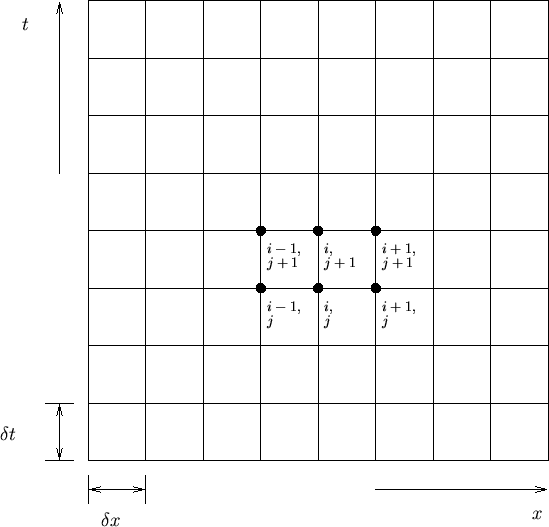
\includegraphics[scale=.45]{imagens/ilustracoes/discretizationFDM.png}
                    \caption{Domínio discretizado \cite{discreteDomainFig}}
                    \label{fig:discreteFDM}
                \end{figure}
                na qual $\delta x$ e $\delta t$ são os tamanhos dos espaços criados nas dimensões da cama elástica, que é o nosso domínio.
                
                Como podemos ver na Figura \ref{fig:discreteFDM}, a discretização do domínio leva à criação de pontos ao longo dele. Esses pontos são indexados na imagem por $i$ (referente à variável $x$) e $j$ (referente à variável $t$). Dessa forma temos que o domínio, agora discreto, do nosso problema é dado por
                \begin{align*}
                    0 \leq  &x_i \leq a\\
                    0 \leq  &t_j \leq b
                \end{align*}.
                
            \subsection{Cálculo}
            
                Tendo sido feita a discretização do domínio do problema, devemos partir para a parte dos cálculos, a ser realizada por meio das fórmulas de diferenças finitas apropriadas. Por exemplo, caso o problema fosse avaliar a função $f''(x)$ no domínio que definimos, deveríamos aplicar uma das fórmulas (\ref{u''Reg}), (\ref{u''Prog}) ou (\ref{u''Cent}) (dependendo de onde o método esteja focado no domínio do problema) para todos os pontos $(x_i, t_j)$ discretizados. Assim, obteríamos uma malha com todos os valores da derivada para todos os pontos.
    
    \chapter{O Método de Traçamento de Raios}

    \label{cap:RT}

    \section{O Funcionamento e a Finalidade}
    
        O traçamento de raios é uma técnica que, basicamente, consiste em modelar a propagação de ondas através de um \textit{meio} elástico utilizando ferramentas chamadas \textit{raios}. 
        
        No caso do traçamento tratado nesse trabalho, consideraremos um modelo de propagação de ondas sísmicas em uma geologia acamadada. Esses raios são emitidos por uma fonte na superfície do meio e traçados, de acordo com uma lei matemática (a ser mostrada na Seção \ref{raySec}), até que alguma camada do meio seja encontrada. Nesse momento, aplica-se a lei de Snell sobre o raio de acordo com a propriedade da camada (se ela é refletora ou transmissora) e inicia-se novamente o traçamento, como se a última camada encontrada fosse a nova fonte. Isso ocorre até que a superfície seja alcançada. Na superfície podem existir receptores que podem ser atingidos pelos raios traçados \cite{notasAulas2017}.
        
        Podemos ter alguma ideia do procedimento descrito acima com a ajuda da Figura \ref{fig:rayTracing}. A fonte emite os raios que atravessam as camadas transmissoras até alcançar a camada refletora previamente definida. A partir daí, os raios sobem até os receptores.
        
        \begin{figure}[H]
            \centering
            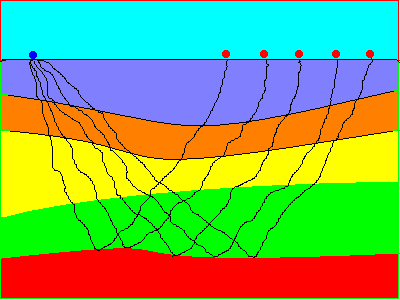
\includegraphics[scale=.8]{imagens/ilustracoes/rayTracing.png}
            
            \hrulefill
            \caption{Imagem meramente ilustrativa sobre o traçamento de raios. O ponto azul representa uma fonte e os pontos vermelhos, receptores. As camadas da subsuperfície são ilustradas pelas cores lilás, laranja, amarelo, verde e vermelho, respectivamente, sendo essa última a camada refletora dos raios e as demais, transmissoras. As linhas pretas que ligam a fonte aos receptores são os raios.}
            \hrulefill
            \label{fig:rayTracing}
        \end{figure}
        
        Existem vários outros tipos de traçamento de raios, podendo-se ter todos os raios emitidos pela fonte refletidos em um único ponto de alguma camada do meio ou todos os raios emitidos refletindo para um único receptor. No geral, todos esses tipos de traçamento de raios visam possibilitar a análise da estrutura de um determinado meio usando-se as propriedades da propagação de ondas para isso \cite{notasAulas2017}.
    
    \section{O Meio}
    
        O meio a ser vasculhado pelo traçamento de raios pode ser formado ou não por camadas. Para esse trabalho, assumimos um meio formado por camadas, sendo essas dispostas uma por cima da outra e com a condição de que uma camada pode ter contato apenas com, no máximo, duas outras. Além disso, consideramos a atmosfera encontrada acima da primeira camada como uma dessas também. Esse meio é uma adaptação do que seria um meio \textbf{acamadado} no ramo da sismologia \cite{notasAulas2017}.
        
        Cada uma das camadas do meio possui como propriedades principais sua espessura, os formatos e posições de suas interfaces (que separam uma camada de outra) e a sua velocidade sísmica, que é ``a taxa pela qual uma onda sísmica viaja através de um meio, que é, a distância dividida pelo tempo de trânsito'' \cite{OilfieldGlossary:seismicVelocity}, sendo o tempo de trânsito a ``duração da passagem de um sinal a partir de uma fonte através da Terra e voltando para um receptor'' \cite{OilfieldGlossary:travelTime}.
        
        Na sismologia, a determinação dessas propriedades das camadas é importante para que se possa cogitar sobre os materiais que formam cada camada e, dependendo da aplicação do método, como esses materiais poderiam ser alcançados fisicamente.
    
    \section{O Raio}
    
        \label{raySec}
        
            Modelar campos de ondas computacionalmente tem um alto custo. Para contornar esse problema, utilizamos a teoria dos raios ao nosso favor. Um raio é como uma parte infinitesimal de uma frente de onda ao longo do tempo, sendo também perpendicular a esta. Um conjunto de raios que simulam partes da mesma frente de onda tomam o formato dela no decorrer do tempo, o que seria possível observar se a propagação da frente de onda fosse simulada por completo. Utilizando apenas pequenas partes (raios) de um domínio muito maior (frente de onda), o traçamento de raios consegue superar a simulação completa no que tange ao custo computacional.
    
            Como dito, o raio simula uma pequena parte de uma frente de onda \textbf{ao longo do tempo}. Ora, mas o que significa a expressão explicitada? Quer dizer que cada ponto do corpo do raio é a posição da parte infinitesimal da frente de onda representada no tempo. Para tentar entender essa questão mais facilmente, veja a Figura \ref{fig:ray&WavePropagation}
            \begin{figure}[H]
                \centering
                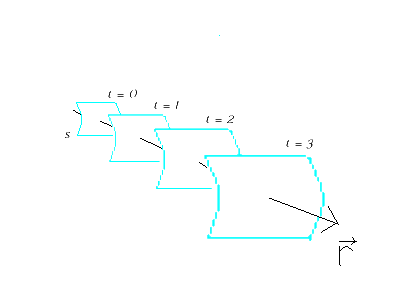
\includegraphics[scale=.8]{imagens/ilustracoes/ray.png}
                \caption{Propagação de uma parte infinitesimal $s$ de uma frente de onda, ao longo do tempo $t$, na direção de um vetor $\vec{r}$. A trajetória do vetor $\vec{r}$ ao longo do tempo forma o raio.}
                \label{fig:ray&WavePropagation}
            \end{figure}
            Imagine que o vetor $\vec{r}$ é sempre perpendicular à frente de onda e a segue. Se traçássemos os pontos de sua trajetória ao longo do tempo, teríamos então um raio e, por ele, a forma como a frente de onda propagou no decorrer do tempo.
            
            \subsection{Uma Brevíssima Visão Sobre a Teoria dos Raios}
            
                A teoria dos raios possui se baseia numa teoria matemática muito complexa e densa, em um nível que foge ao escopo desse trabalho. Por isso, explicaremos do que se trata essa teoria da forma mais básica possível.
                
                Assumamos ondas de alta frequência. Sabemos que a equação da onda é algo como 
                \begin{equation}
                    \label{eqOndaRaySec}
                    \nabla^2u(\vec{x}, t) - \dfrac{1}{\alpha^2}\dfrac{\partial^2u(\vec{x}, t)}{\partial t^2} = 0
                \end{equation}
                onde $\nabla^2$ é o operador laplaciano, que representa
                \begin{equation}
                    \nabla^2 = \dfrac{\partial^2}{\partial x^2} + \dfrac{\partial^2}{\partial y^2}
                \end{equation}
                para o caso de duas dimensões espaciais e $\vec{x}$ é o vetor posição em $x$ e $y$. Então, se assumirmos uma solução harmônica como
                \begin{equation}
                    u(\vec{x}, t) = A(\vec{x})e^{-i\omega(T(\vec{x}) + t)}
                \end{equation}
                na qual $\omega$ é a frequência da onda, $A(\vec{x})$ é a amplitude de uma determinada posição $(x, y)$ da onda e $T(\vec{x}) = c$ é uma frente de onda (o $\nabla T$ define o \textit{raypath}, ou seja, uma linha, sempre perpendicular à frente de onda no caso dos meios isotrópicos, que define as direções que a propagação da onda assumiu \cite{OilfieldGlossary:raypath}), e, usando as derivadas da solução, realizarmos as devidas substituições e manipulações na equação da onda \ref{eqOndaRaySec} teremos que a equação resultante pode ser separada em suas partes real e imaginária \cite{RawlinsonSlide06_RayTheory}.
                
                A parte real,
                \begin{equation}
                    \nabla^2A - \omega^2A|\nabla T|^2 = \dfrac{-A\omega^2}{\alpha^2}
                \end{equation}
                que, ao ser dividida por $A\omega^2$ e levando-se em conta a hipótese de ondas de alta frequência ($\omega \rightarrow \infty$), leva à \textbf{equação iconal}
                \begin{equation}
                    \label{eikonalEquation}
                    |\nabla T| = \dfrac{1}{\alpha^2}
                \end{equation}
                que ``descreve a propagação cinemática de ondas de alta frequência'' \cite{RawlinsonSlide06_RayTheory} (tradução nossa). O lado direito dessa equação, $\dfrac{1}{\alpha^2}$, é chamado \textbf{vagarosidade} \cite{RawlinsonSlide06_RayTheory}. Já a parte imaginária,
                \begin{equation}
                    2\omega\nabla A\cdot\nabla T + \omega A\nabla^2T = 0
                \end{equation}
                ao ser dividida por $\omega$, leva a \textbf{equação de transporte},
                \begin{equation}
                    2\nabla A\cdot\nabla T + A\nabla^2T = 0
                \end{equation}
                que ``pode ser usada para computar a amplitude das ondas que estão propagando'' \cite{RawlinsonSlide06_RayTheory}.
                
                Da equação iconal (\ref{eikonalEquation}), utilizando o processo aplicado em \cite{Miqueles2006}, obtemos o sistema de equações 
                \begin{align}
                    \dfrac{d\vec{x}}{dT} &= v(x)^2\vec{p}\\
                    \dfrac{d\vec{p}}{dT} &= \dfrac{1}{v(x)}\nabla v(\vec{x})
                \end{align}
                nas quais, $\vec{p}$ é chamado \textbf{vetor vagarosidade}. A solução desse sistema é algo no formato $(\vec{x}, \vec{p})$, sendo $\vec{x}$, quando o problema é resolvido computacionalmente, um \textit{array} de alguns dos pontos pelos quais o raio passou. Já $\vec{p}$ é um \textit{array} de algumas direções assumidas pelo raio ao longo do traçamento \cite{Miqueles2006}. Digo algumas porque a solução analítica possui infinitos pontos e infinitas direções durante o traçamento, mas isso não ocorre computacionalmente.
    
    \chapter{Equação da Onda em Meios Não-Homogêneos}

    \label{cap:CompMDFeRT}

    \section{Resolução da Equação da Onda por Diferenças Finitas}
    
        Como já dito, o objetivo desse trabalho é a comparação de métodos que consigam resolver a equação da onda com fonte, 
        simulando a propagação de oscilações através de meios acamadados de composição não-homogênea. Portanto, 
        seguindo o escopo desse objetivo, apresentaremos nesse relatório apenas as simulações para o caso em duas 
        dimensões das oscilações, como se dá no estudo da sísmica.
    
        \subsection{Reflexão na Borda do Domínio de Propagação da Onda}
	        
            Suponhamos um meio acamadado cujas interfaces, na forma de retas que podem ser representadas por funções, 
            se distribuem como na figura abaixo:
            \begin{figure}[H]
                \centering
                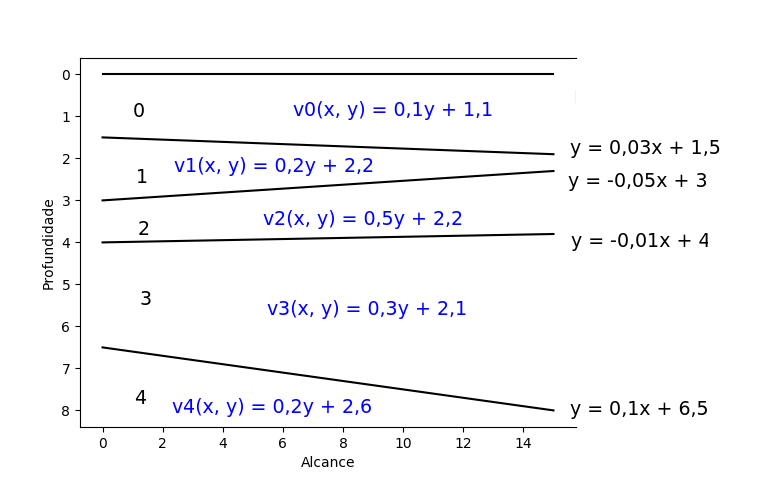
\includegraphics[scale=.7]{imagens/ilustracoes/TR.png}
                \caption{Meio acamadado com interfaces retas (em preto) representadas por funções e camadas representadas
                por números de 0 a 4. As funções de velocidade de cada camada também são apresentadas na imagem}
                \label{fig:interfacesAndMedium}
            \end{figure}
            Além da distribuição das interfaces, a imagem também apresenta como se dá a propriedade de não-homogeneidade do 
            meio através das funções de velocidades para cada camada. Em um ambiente real, a não-homogeneidade se dá através 
            da formação das camadas por diversos tipos de materiais que estão misturados e cuja distribuição depende da posição 
            em que se encontram e da pressão que sofrem.
            
            As bordas do meio definido refletem as ondas. Para tal, podemos pensar o meio por onde a onda propagará como uma
            cama elástica, que é presa em suas bordas. Para imitar isso, usamos as condições de contorno como em (\ref{eq:condContorno})
            que pode ser implementado em código: imagine um \textit{array} tridimensional (visto que o problema se dá em $x$, $y$ e $t$)
            no qual, para cada posição no eixo que representa $t$ exista um \textit{array} $xy$ que representa o nosso meio. Então aplicamos as
            condições de contorno zerando as ``bordas'' de cada um desses arrays.
            
            Para que simulemos o espalhamento das oscilações precisamos de uma fonte as inicie. Para isso, podemos utilizar a \textit{wavelet} 
            de Ricker (também conhecida como \textit{mexican hat wavelet}) como fonte. Essa \textit{wavelet} é dada pela função
            \begin{equation}
                \label{eq:rickerWavelet}
                f(t) = (1 - 2\pi^2f_M^2t^2)^{-\pi^2f_M^2t^2}
            \end{equation}
            na qual, $t$ representa o tempo e $f_M$ representa a frequência de pico \cite{rickerWLet}. Podemos visualisar um exemplo da \textit{wavelet} na Figura \ref{fig:Ricker}
            \begin{figure}[H]
                \centering
                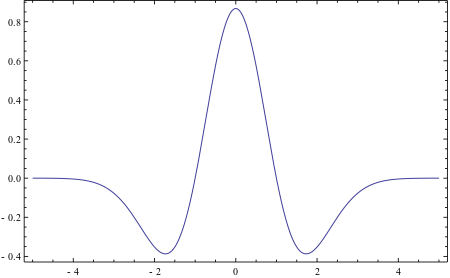
\includegraphics[scale=.6]{imagens/MexicanHatMathematica.png}
                \caption{Exemplo da \textit{wavelet} de Ricker, por JonMcLoone [CC BY-SA 3.0 (https://creativecommons.org/licenses/by-sa/3.0)], via Wikimedia Commons}
                \label{fig:Ricker}
            \end{figure}
            
            Suponhamos também que esse meio está englobado por um sistema de coordenadas cartesianas cuja origem se encontra
            no extremo esquerdo superior da imagem (\ref{fig:interfacesAndMedium}) e cujo eixo das ordenadas aponta para baixo. 
            Assume-se o eixo assim porque a simulação da propagação de ondas se dará por todo o meio, que é subterrâneo, e para 
            baixo.
	        
            \subsubsection{Prática Numérica}
            
                Utilizando o arquivo \textit{userInput.py}, recebemos os parâmetros para a onda e o meio que o usuário deseja que a simulação siga, gerando um arquivo \textit{data.npy}. Após isso executamos o arquivo \textit{reflect.py}, que lerá o arquivo \textit{data.py}, criará o meio e a onda como desejado e realizará a simulação usando o método de diferenças finitas. Por fim o programa salva um arquivo \textit{U.npy}, que contém a simulação da propagação de ondas. Esse último arquivo pode ser usado pelo programa \textit{snapshoter.py} para gerar \textit{snapshots} (``fotografias'') das superfícies de contorno da onda.
                
                Os \textit{snapshots} da Figura \ref{fig:snapsMDF} foram criados para uma simulação da propagação, com no máximo 90 s, de uma onda com frequência dominante de um hertz, amplitude de um quilômetro, pico da fonte na origem do meio que tem 15 km de extensão e 9,5 km de profundidade. As velocidades do meio se distribuem de acordo com o que podemos ver na imagem \ref{fig:velDist}.
                
                \begin{figure}[H]
                    \centering    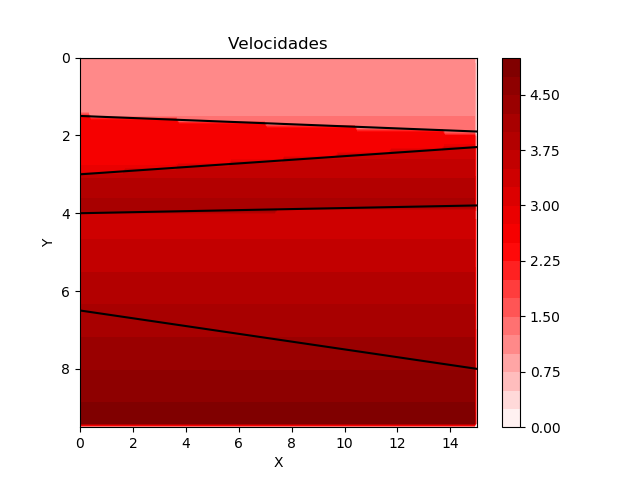
\includegraphics[scale=.8]{imagens/FDMimages/Velocidades.png}
                    \caption{Distribuição das velocidades no meio usado como exemplo}
                    \label{fig:velDist}
                \end{figure}
                
                \begin{figure}[H]
                    \begin{tabular}{cc} 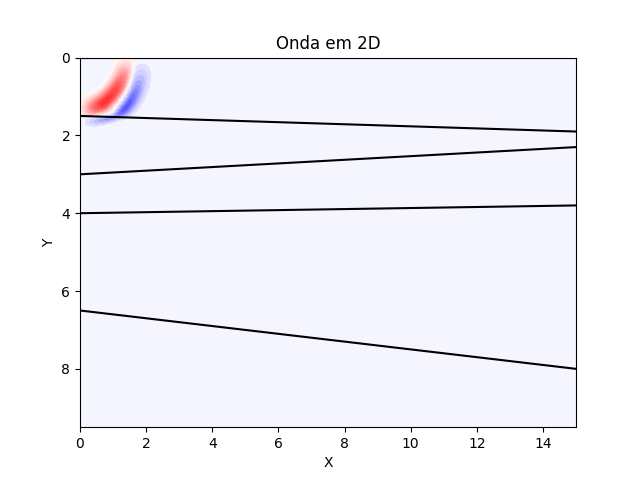
\includegraphics[width=65mm]{imagens/FDMimages/Teste00.png} &  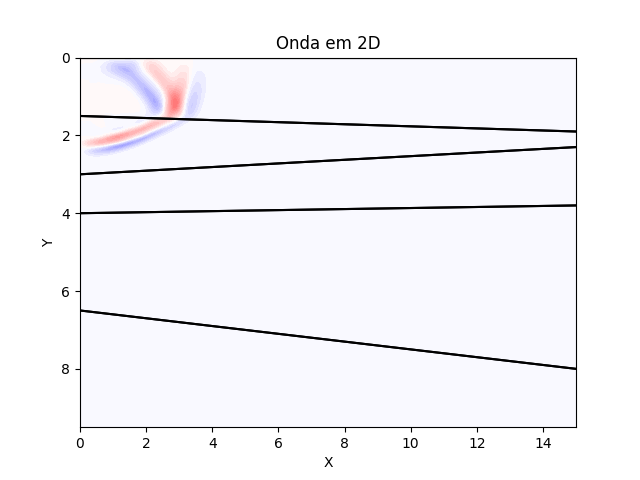
\includegraphics[width=65mm]{imagens/FDMimages/Teste01.png} \\
                    (a) 1 & (b) 2 \\
                    [6pt] 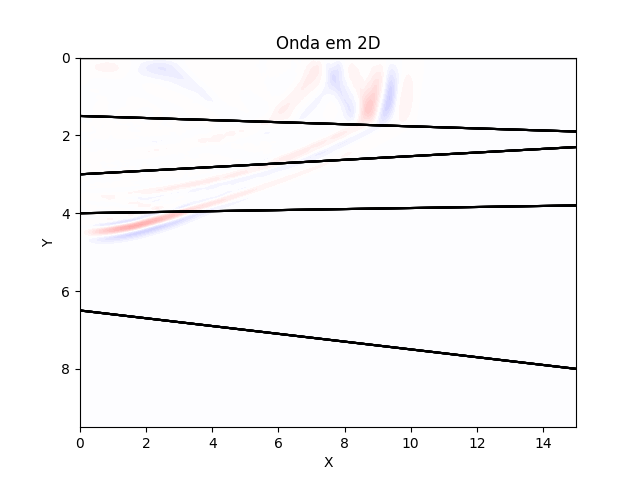
\includegraphics[width=65mm]{imagens/FDMimages/Teste05.png} & 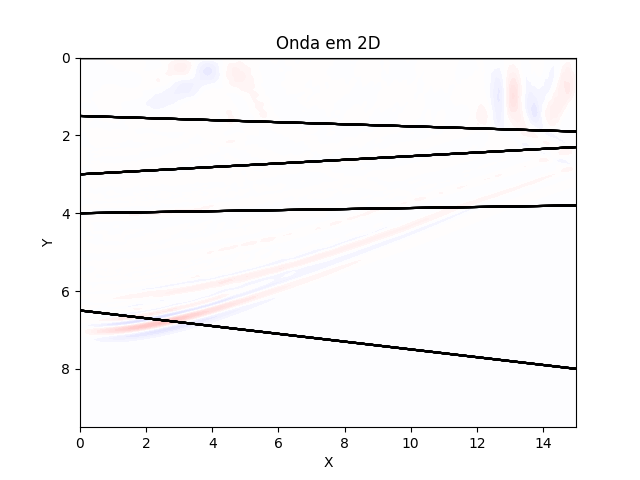
\includegraphics[width=65mm]{imagens/FDMimages/Teste010.png} \\
                    (c) 3 & (d) 4 \\
                    [6pt] 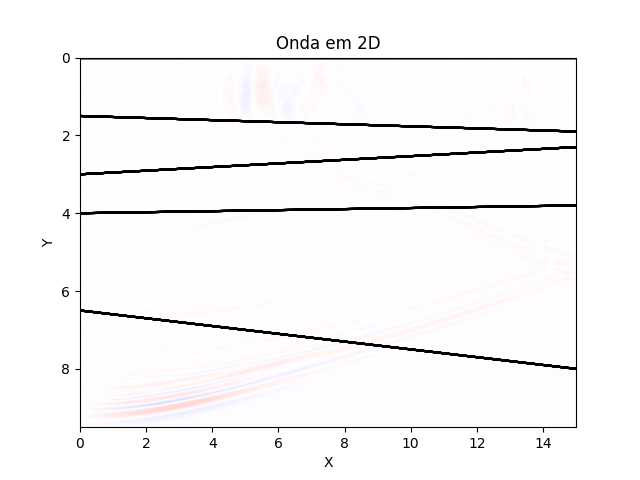
\includegraphics[width=65mm]{imagens/FDMimages/Teste015.png} & 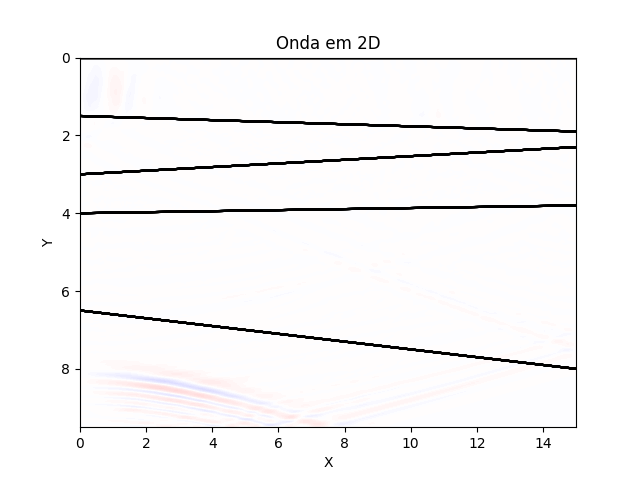
\includegraphics[width=65mm]{imagens/FDMimages/Teste019.png} \\ 
                    (e) 5 & (f) 6\\
                    [6pt] 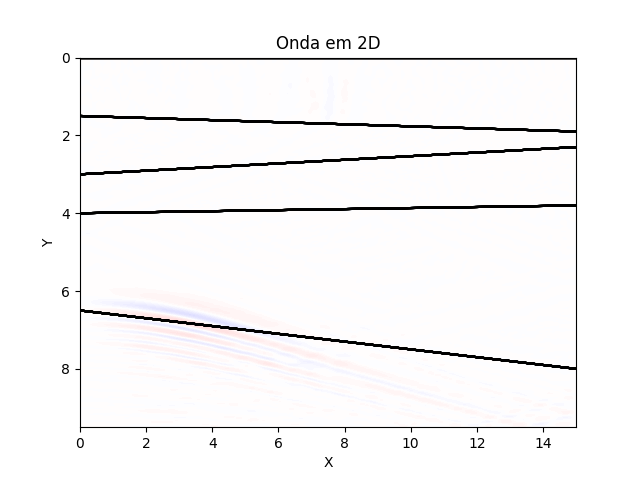
\includegraphics[width=65mm]{imagens/FDMimages/Teste023.png} &  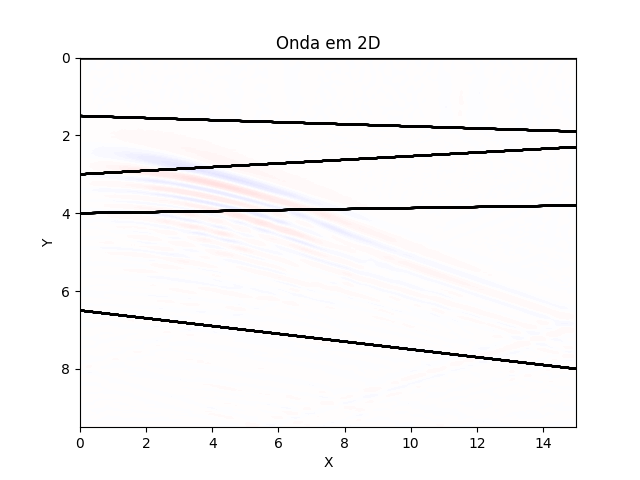
\includegraphics[width=65mm]{imagens/FDMimages/Teste030.png}\\
                    (e) 7 & (f) 8
                    \end{tabular}
                    \caption{\textit{Snapshots} da simulação numérica da propagação de uma onda}
                    \label{fig:snapsMDF}
                \end{figure}

                Na Figura \ref{fig:snapsMDF} podemos perceber que, como vimos no Capítulo \ref{cap:ond}, a cada vez que a onda encontra uma outra função de velocidades, ocorre uma refração e uma reflexão da onda. Por uma falha não ocorrem refrações e reflexões significantes nas camadas 3 e 4 pois, como se pode ver na Figura \ref{fig:velDist}, o gradiente de velocidades dessas camadas parece ser o mesmo.

	    \subsection{Domínio com Bordas ``Absorventes''}
	        
            Existem várias sugestões de implementações do método de diferenças finitas para a equação da onda com condições de contorno ``absorventes'' (ou ``abertas''). 
            
            Expandiremos o domínio de simulação de propagação das ondas, mas apresentaremos nas imagem apenas a parte que nos interessa. Dessa forma, durante a sua propagação, a onda não refletirá nas bordas da imagem como na seção anterior, mas dará a impressão de sair pelas bordas dela.
	        
            \subsubsection{Prática Numérica}
            
                Utilizando a mesma distribuição de velocidades visto na Figura \ref{fig:velDist}, obtemos a simulação demonstrada pelos \textit{snapshots} da Figura \ref{snapsMDFAbs}. Pode-se perceber que, ao contrário do caso das bordas refletoras, no caso atual, as frentes de onda passam além das extremidades da parte do meio que foi exibida. É como se o primeiro caso fosse um corpo caindo numa bacia de água, com o tempo, a superfície da possui um comportamento ondulatório complexo, com várias ondas se sobrepondo. Já o segundo o caso é como se o corpo caísse sobre a superfície do mar, onde não haveria bordas para as reflexões. Isso desconsiderando as reflexões que surgem com a passagem da frente de onda de uma camada para outra.
                
                \begin{figure}[H]
                    \begin{tabular}{cc}
                        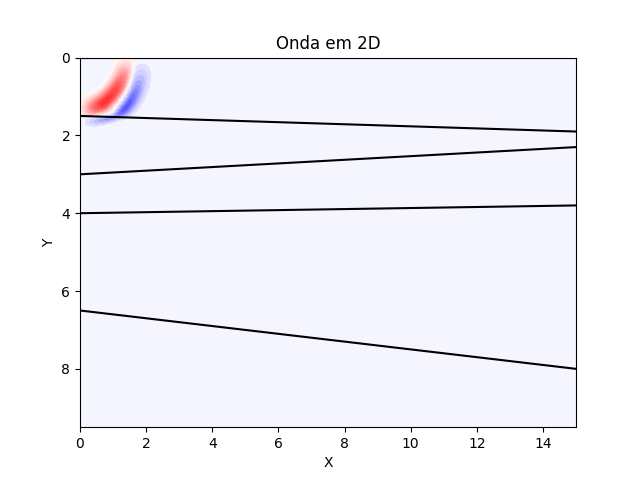
\includegraphics[width=65mm]{imagens/FDMimages/Teste00.png} & 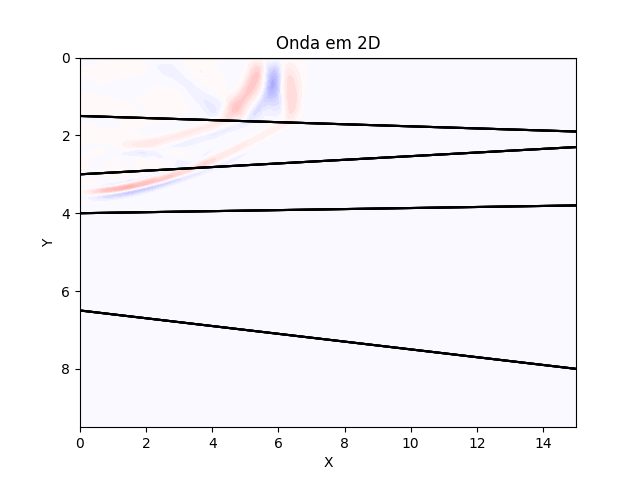
\includegraphics[width=65mm]{imagens/FDMimages/Teste03.png} \\
                        (a) 1 & (b) 2 \\
                        [6pt] 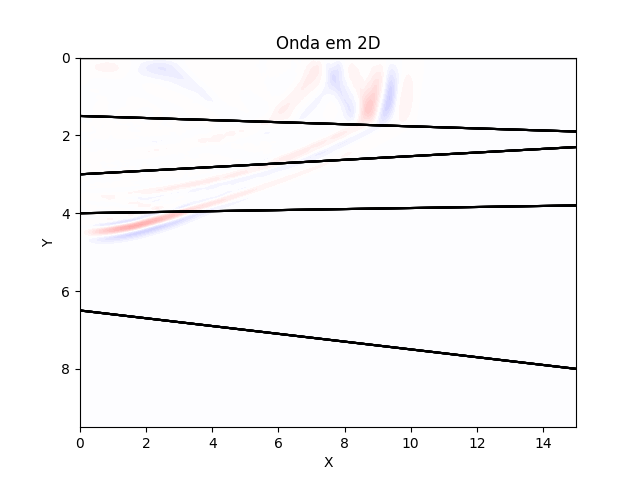
\includegraphics[width=65mm]{imagens/FDMimages/Teste05.png} & 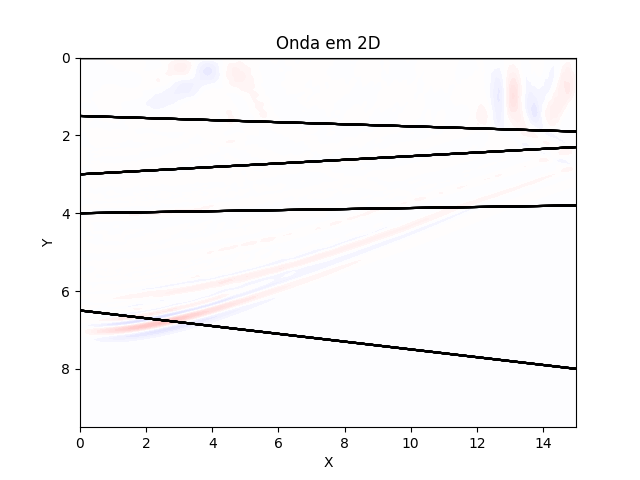
\includegraphics[width=65mm]{imagens/FDMimages/Teste010.png} \\
                        (c) 3 & (d) 4 \\
                        [6pt] 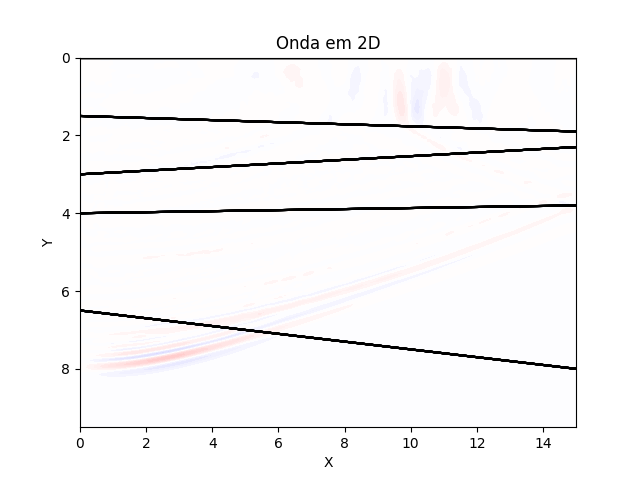
\includegraphics[width=65mm]{imagens/FDMimages/Teste012.png} & 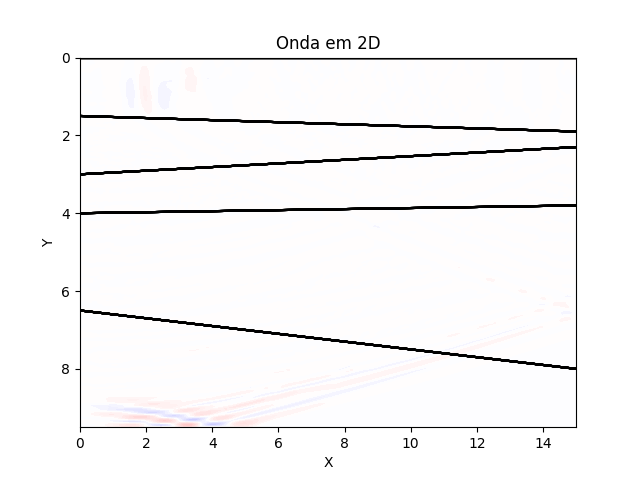
\includegraphics[width=65mm]{imagens/FDMimages/Teste017.png} \\ 
                        (e) 5 & (f) 6\\
                        [6pt] 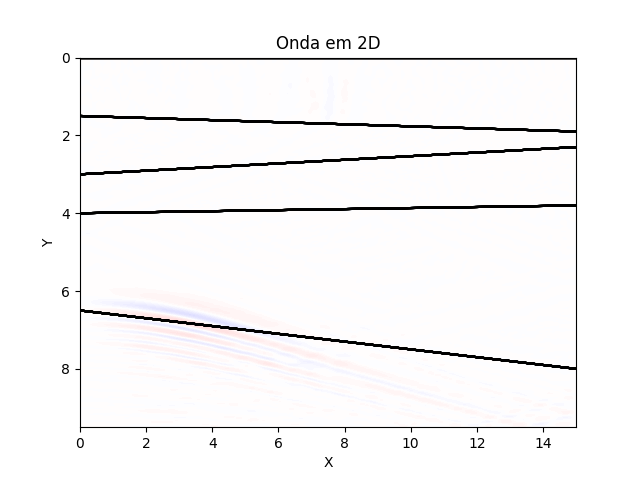
\includegraphics[width=65mm]{imagens/FDMimages/Teste023.png} & 
                        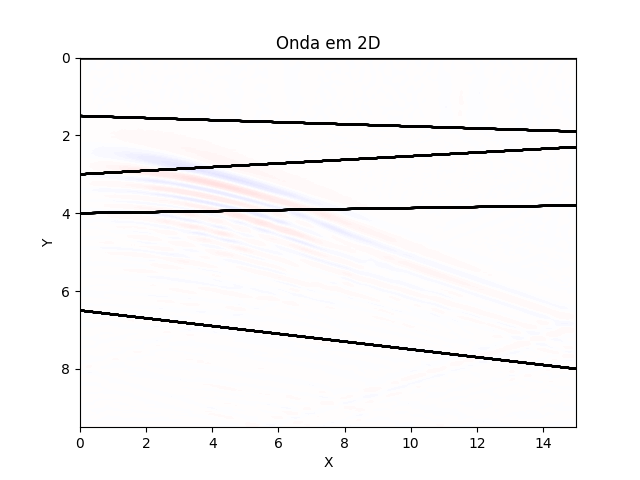
\includegraphics[width=65mm]{imagens/FDMimages/Teste030.png}\\
                        (e) 7 & (f) 8
                    \end{tabular}
                    \caption{\textit{Snapshots} da simulação numérica da propagação de uma onda.}
                    \label{snapsMDFAbs}
                \end{figure}

            
    \section{Resolução da Equação da Onda pelo Traçamento de Raios}
    
        \subsection{Implementação}
        
            Foi implementado um traçamento de raios simples, no qual há apenas uma reflexão nas interfaces que são definidas como refletoras. Neste traçamento, não são representadas as reflexões que ocorrem com as refrações.
            
            O raio é implementado como um \textit{array} de pontos que indicam sua posição $(x, y)$ no tempo $t$ e outro \textit{array} de componentes que constituem o vetor direção do raio ao longo do tempo. Já as interfaces são implementadas como retas em sua forma paramétrica: com um vetor diretor e um ponto. Além disso, a interface também possui um vetor normal.
        
            \subsubsection{O Traçamento}
            
                As posições e direções do raio ao longo do tempo são calculadas com o auxílio do método de Runge-Kutta de quarta ordem. Isso é feito porque o raio é definido matematicamente como um sistema de equações diferenciais para a posição e a direção ao longo do tempo.
                
                A interseção do raio com com a próxima interface se dá da seguinte forma: quando a função que implementa o método de Runge-Kutta percebe que o raio ultrapassou a interface, ela cria uma reta ligando os dois últimos pontos traçados para o raio e calcula a interseção dessa reta com a interface. O ponto de interseção calculado torna-se o último ponto do traçamento do raio para aquela camada.
            
            \subsubsection{Lei de Snell}
            
                Temos que a lei de Snell se dá por
                \begin{equation*}
                    \dfrac{\sin{\theta_2}}{\sin{\theta_1}} = \dfrac{v_2}{v_1} = \dfrac{n_1}{n_2}
                \end{equation*}
                na qual, $\theta_1$ e $\theta_2$ são os ângulos que, respectivamente, os raios incidente e refratado fazem com a normal, $v_1$ e $v_2$ são as velocidades dos meios acima e abaixo da reta preta (nas Figuras \ref{fig:reflect} e \ref{fig:refract}), respectivamente, assim como $n_1$ e $n_2$ são os coeficientes de refração de cada um, também respectivamente. A implementação da reflexão e da refração se baseiam nessa lei.
                
            \subsubsection{A Reflexão}
            
                Estando o raio sobre a interface que ele deve refletir, calculamos a projeção vetorial, $\vec{s}$, do último vetor direção, $\vec{p}$, do raio sobre a normal da interface. Após isso, somamos $\vec{p}$ com menos duas vezes $\vec{s}$ e obtemos o vetor direção refletido do raio. Também podemos visualizar isso pela seguinte imagem.
                
                \begin{figure}[H]
                    \centering 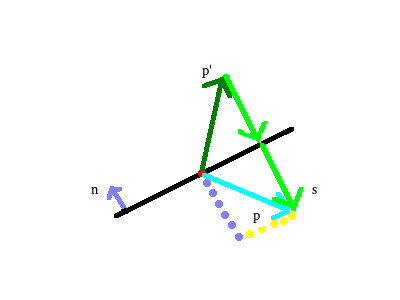
\includegraphics[scale=.8]{imagens/RTimages/reflect.png}
                    \caption{Esquema ilustrativo da reflexão do raio $\vec{p}$, em azul ciano, sobre uma interface, em preto. O vetor $\vec{s}$, em verde, é a projeção vetorial de $\vec{p}$ sobre o vetor normal $\vec{n}$ da interface, em lilás}
                    \label{fig:reflect}
                \end{figure}
            
            \subsubsection{A Refração}
            
                Estando o raio sobre uma interface não refletora, projetamos o vetor $\vec{p}$ sobre o vetor diretor $\vec{d}$ da interface. Dessa forma, sendo $\vec{p}$ um vetor unitário, obtemos o seno do ângulo da direção do raio naquele momento pela norma do vetor projetado. Com esse seno, aplicamos a lei de Snell e obtemos o seno do ângulo refratado. Então, pela seguinte igualdade trigonométrica
                \begin{equation*}
                    \cos{\theta} = \sqrt{1 - \sin^2{\theta}}
                \end{equation*}
                obtemos o cosseno do ângulo refratado. Assim, podemos multiplicar vetor $\vec{n}$ da interface pelo cosseno encontrado e somar esse vetor a $\vec{d}$ multiplicado pelo seno, obtendo então o novo vetor $\vec{p}$ do raio.
                
                \begin{figure}[H]
                    \centering
                    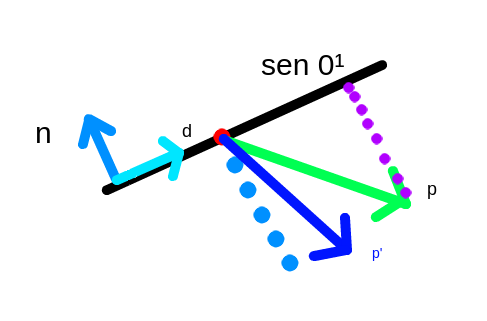
\includegraphics[scale=.6]{imagens/RTimages/refract.png}
                    
                    \hrulefill
                    \caption{Esquema ilustrativo da reflexão do raio $\vec{p}$, em verde, sobre uma interface, em preto. A norma da projeção de $\vec{p}$ sobre $\vec{d}$, em azul claro, é o seno do ângulo de $\vec{p}$ com a normal $\vec{n}$, em azul escuro. Após a aplicação da lei de Snell sobre esse seno, obtém-se o seno do ângulo refratado, que é usado para obter o cosseno do mesmo ângulo. Obtém-se $\vec{p'}$ multiplicando o cosseno e o seno encontrados por $\vec{n}$ e $\vec{d}$, respectivamente}
                    \hrulefill
                    \label{fig:refract}
                \end{figure}
            
        \subsection{Traçando Raios}
        
	        Utilizando a mesma distribuição de velocidades usada nos exemplos de implementação do método de diferenças finitas, podemos ver abaixo a simulação da propagação de ondas pelo mesmo meio das outras simulações, mas agora pelo método de traçamento de raios. Os ângulos mínimo e máximo de emisão dos raios foram, respectivamente, 10º e 18º. A cada encontro do raio com uma interface podemos ver uma refração (calculada usando a função velocidade das duas camadas naquele ponto), exceto na última interface.
	        
            \begin{figure}[H]
            	\centering
            	\label{RTsim01}
            	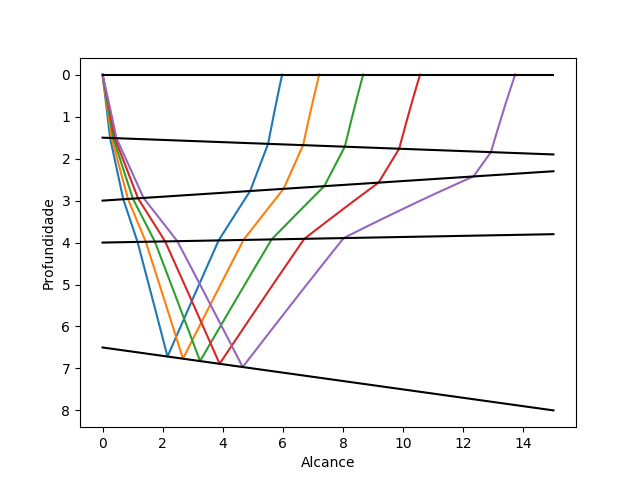
\includegraphics[scale=.6]{imagens/RTimages/sim01.png}
            	\caption{Simulação da propagação de ondas pelo método do traçamento de raios}
            \end{figure}
            
            \begin{figure}[H]
               	\centering
               	\label{RTsim02}
               	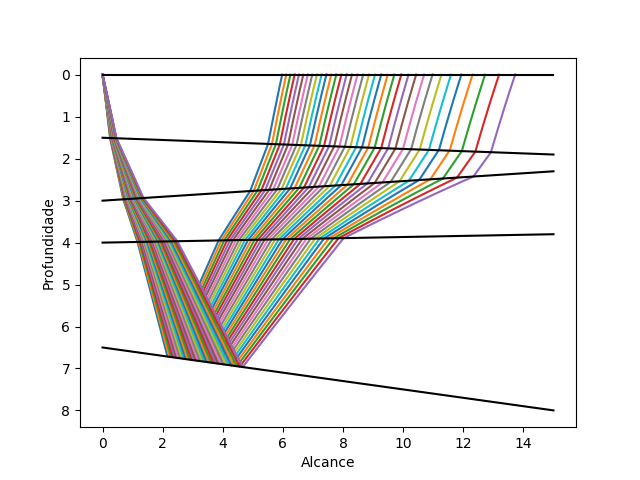
\includegraphics[scale=.6]{imagens/RTimages/sim02.png}
               	\caption{A mesma simulação que a Figura \ref{RTsim01} exibe, mas agora com 35 raios}
            \end{figure}
            
            \newpage
            Podemos ver pelas simulações seguintes que é também possível decidir sobre qual interface os raios devem refletir. Isso é útil para se observar como se dá a reflexão sobre cada interface
            \begin{figure}[H]
               	\centering
               	\label{RTsim03}
               	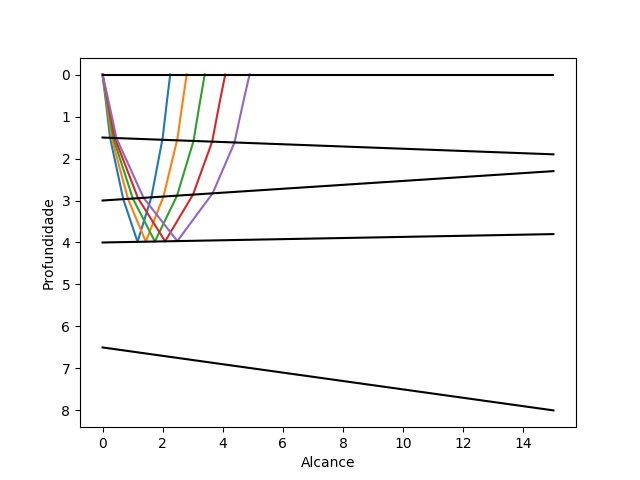
\includegraphics[scale=.6]{imagens/RTimages/sim03.png}
               	\caption{Traçamento de raios com reflexão na terceira interface}
            \end{figure}
            
			\begin{figure}[H]
               	\centering
               	\label{RTsim04}
               	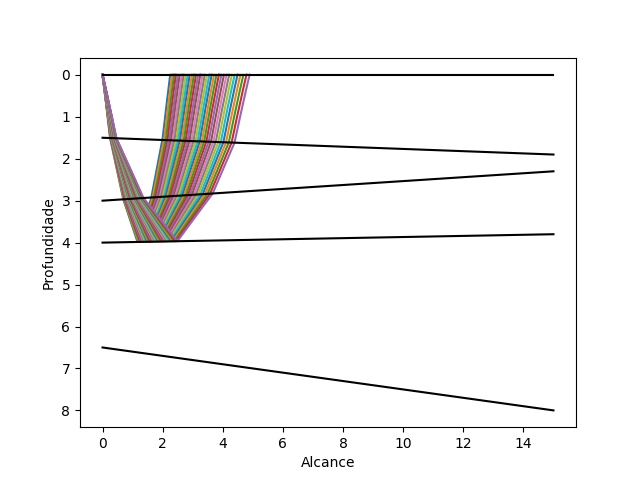
\includegraphics[scale=.6]{imagens/RTimages/sim04.png}
               	\caption{O mesmo traçamento da Figura \ref{RTsim03}, mas agora com mais raios}
			\end{figure}
            
    \section{Comparação Entre os Métodos}
    
        Tanto o método de diferenças finitas quanto o traçamento de raios possuem suas vantagens e desvantagens. Durante a execução deste trabalho pude notar as seguintes características sobre cada uma dessas abordagens para a simulação de propagação de ondas.
        
        \subsection{Método das Diferenças Finitas}
        
            Possui uma forma fácil de se implementar, necessitando-se apenas conhecer os conceitos de derivadas parciais e diferenças finitas, que são relativamente fáceis. Para para a resolução numérica de um problema de equações diferenciais parciais, como a da onda, bastam poucas linhas de código. O uso da biblioteca \textit{Numpy} possibilita isso, além de acelerar os tratamentos numéricos no processo.
            
            Além disso, o a visualização da transformação dos dados, através do tempo, possibilitada método e pelas bibliotecas gráficas permite entender, intuitivamente, que a equação da onda é um modelo que imita bem o fenômeno físico. Essa visualização, em pequena escala, poderia ser utilizada na ministração de aulas de Cálculo Numérico, Métodos Numéricos Computacionais e/ou Física.
            
            Contudo, o processo de simulação por esse método tem um preço alto para grandes domínios (bem como da visualização gráfica de seus dados, que pode custar mais ainda). É comum que, para evitar instabilidades numéricas tenha-se que aumentar o número de pontos no \textit{array}, para que os passos dados pelo método não sejam muito grandes. Isso afeta a quantidade de memória e de processamento (e, consequentemente, de tempo e de recursos financeiros) necessária para a execução da simulação a tal ponto que, para uma simulação na área de Sismologia, por exemplo, que tem um grande volume de dados, a utilização do método se torna inviável.
            
        \subsection{Traçamento de Raios}
        
            A teoria do traçamento de raios é, matematicamente, complicada e nada intuitiva nos primeiros contatos. A implementação em código do traçamento também segue isso, sendo repleta de condicionais e cuidados que devem ser levados em conta. É necessária uma boa compreensão da teoria matemática antes da implementação do método, bem como a paciência com os erros que aparecerão e tempo para a implementação dos detalhes do traçamento.
            
            Contudo, imitar uma parte infinitesimal da frente de onda ao invés de simulá-la completamente é muito mais eficiente e menos custoso. Ou seja, o uso do traçamento de raios gasta menos memória (basta armazenar, além do meio e suas informações, as informações dos raios) e processamento (não é necessária computação sobre um grande \textit{array} tridimensional, mas apenas os \textit{arrays} de posição e direção dos raios) que o método de diferenças finitas para fazer, fundamentalmente, a mesma coisa. É por isso que o traçamento é uma das técnicas mais utilizadas nos ramos como a já citada Sismologia.
            
            Por fim, até mesmo a exibição gráfica dos dados do traçamento, pelo menos em pequena escala como feito nesse projeto, é mais rápida do que no caso da exibição dos dados conseguidos pelo método anterior, visto que exibe-se ``linhas'' e não malhas inteiras.
    
    \chapter{Conclusão}

    \label{cap:concl}
    
    Para alcançar o objetivo proposto de se comparar os métodos de diferenças finitas e traçamento de raios para a simulação da propagação de ondas em meios não-homogêneos foi necessário o estudo não só dos métodos em si, mas dos assuntos que dão base a eles:
    \begin{itemize}
        \item \textbf{Computação numérica}: era necessária a implementação computacional dos métodos numéricos, sendo preciso o entendimento sobre a aritmética computacional e os erros envolvidos em modelagens matemáticas implementadas em computadores;
        \item \textbf{Equações diferenciais parciais}: a teoria de raios assume o raio como uma EDO, sendo necessário o entendimento sobre esse tipo de equação;
        \item \textbf{Resolução numérica de problemas de valor inicial}: visto que o raio é, matematicamente, uma EDO e o traçamento de raios é implementado computacionalmente, é necessário se conhecer como se dá a resolução numérica de EDO's, usando-se, por exemplo, o método de Runge-Kutta;
        \item \textbf{Ondulatória}: para se entender a propagação de ondas é preciso se entender o comportamento delas;
        \item \textbf{Equações Diferenciais Parciais (e a equação da onda)}: a equação da onda é uma EDP e precisamos entendê-la tanto para aplicar o método de diferenças finitas sobre ela, quanto para entender a teoria dos raios.
    \end{itemize}
    
    A partir daí vimos as ideias dos métodos envolvidos na comparação:
    \begin{itemize}
        \item \textbf{Método da diferenças finitas}: modela-se o domínio a ser estudado como uma malha subdividida em retângulos ou paralelepípedos e, para cada ponto dessa malha, aplica-se alguma fórmula (específica para o problema) de diferenças finitas, que são modelagens computacionais para as derivadas;
        \item \textbf{Traçamento de raios}: ao invés de se modelar toda a frente de onda, separa-se uma fração infinitesimal dela e determina-se a posição e a direção dessa fração dentro de um período de tempo previamente determinado.
    \end{itemize}
    Comparando-se as características observadas para cada método, vimos que o traçamento de raios é mais rápido e menos custoso que o método de diferenças finitas, entretanto, a teoria dos raios não é tão intuitiva quando a definição de diferenças finitas.
    
    Esse trabalho me possibilitou enxergar aplicações das disciplinas de Cálculo e Física, bem como da programação, no mundo real. Os estudos realizados durante o projeto permitiram a aquisição de novos conhecimentos sobre ondas (sua presença e aplicações em lugares inusitados, como o estudo do interior da Terra), equações diferenciais e na forma como elas podem ser modeladas para resolver problemas nas áreas das Ciências Exatas e Engenharias. Além disso, pude perceber a necessidade da otimização de modelagens numéricas computacionais, para que sejam resolvidas mais rapidamente e com custo menor, dada a sua importância.
    
    Por fim, o trabalho pode ser melhorado com, por exemplo, uma análise mais técnica da complexidade e do tempo de execução dos programas envolvidos. Além disso, podem ser estudados alguns instrumentos da Sismologia, como os traços sísmicos ou variações do traçamento de raios, como pode ser visto em \cite{Miqueles2006}. Também pode ser feita a otimização dos programas principais envolvidos, como por programação paralela e com técnicas de computação de alto desempenho.
    
    \begin{appendices}
        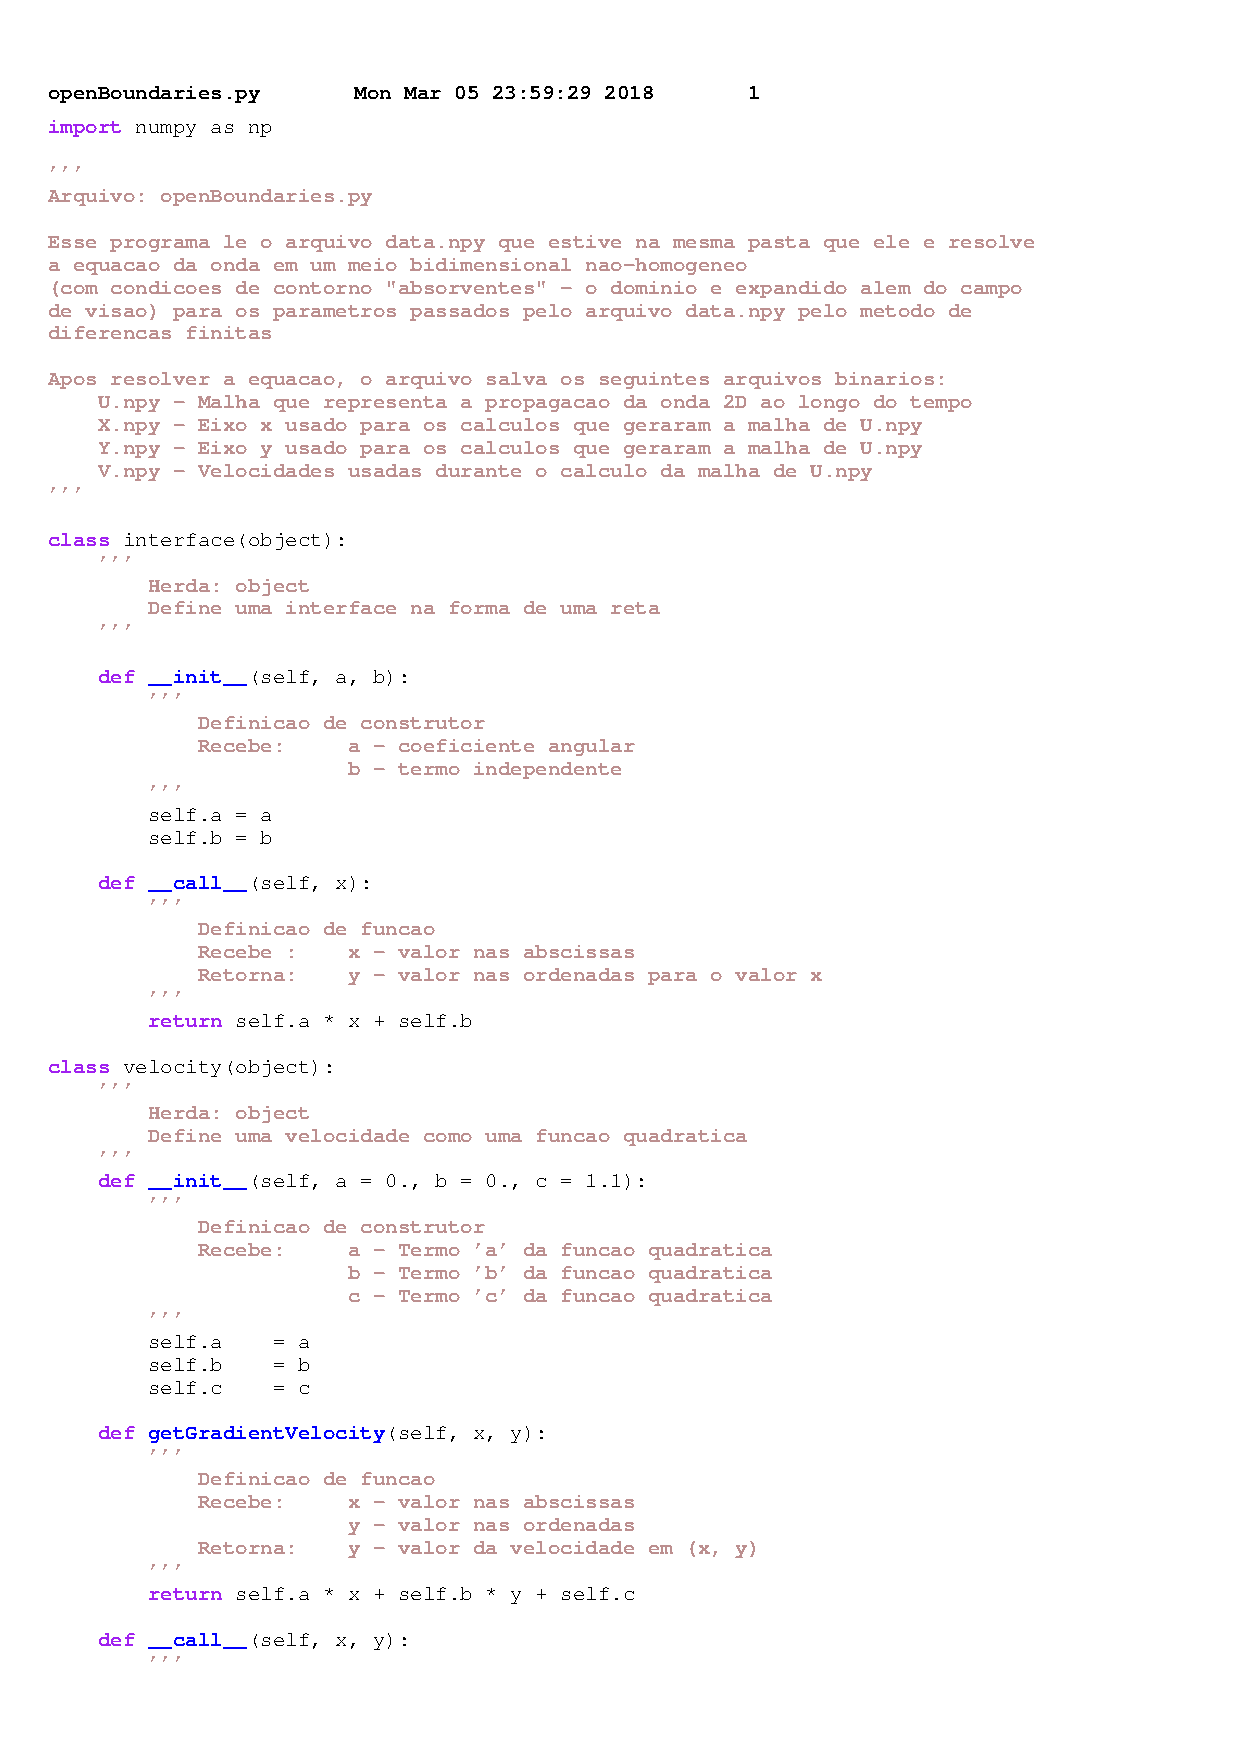
\includepdf[pages=-]{Codigos/FDM/MDF.pdf}
        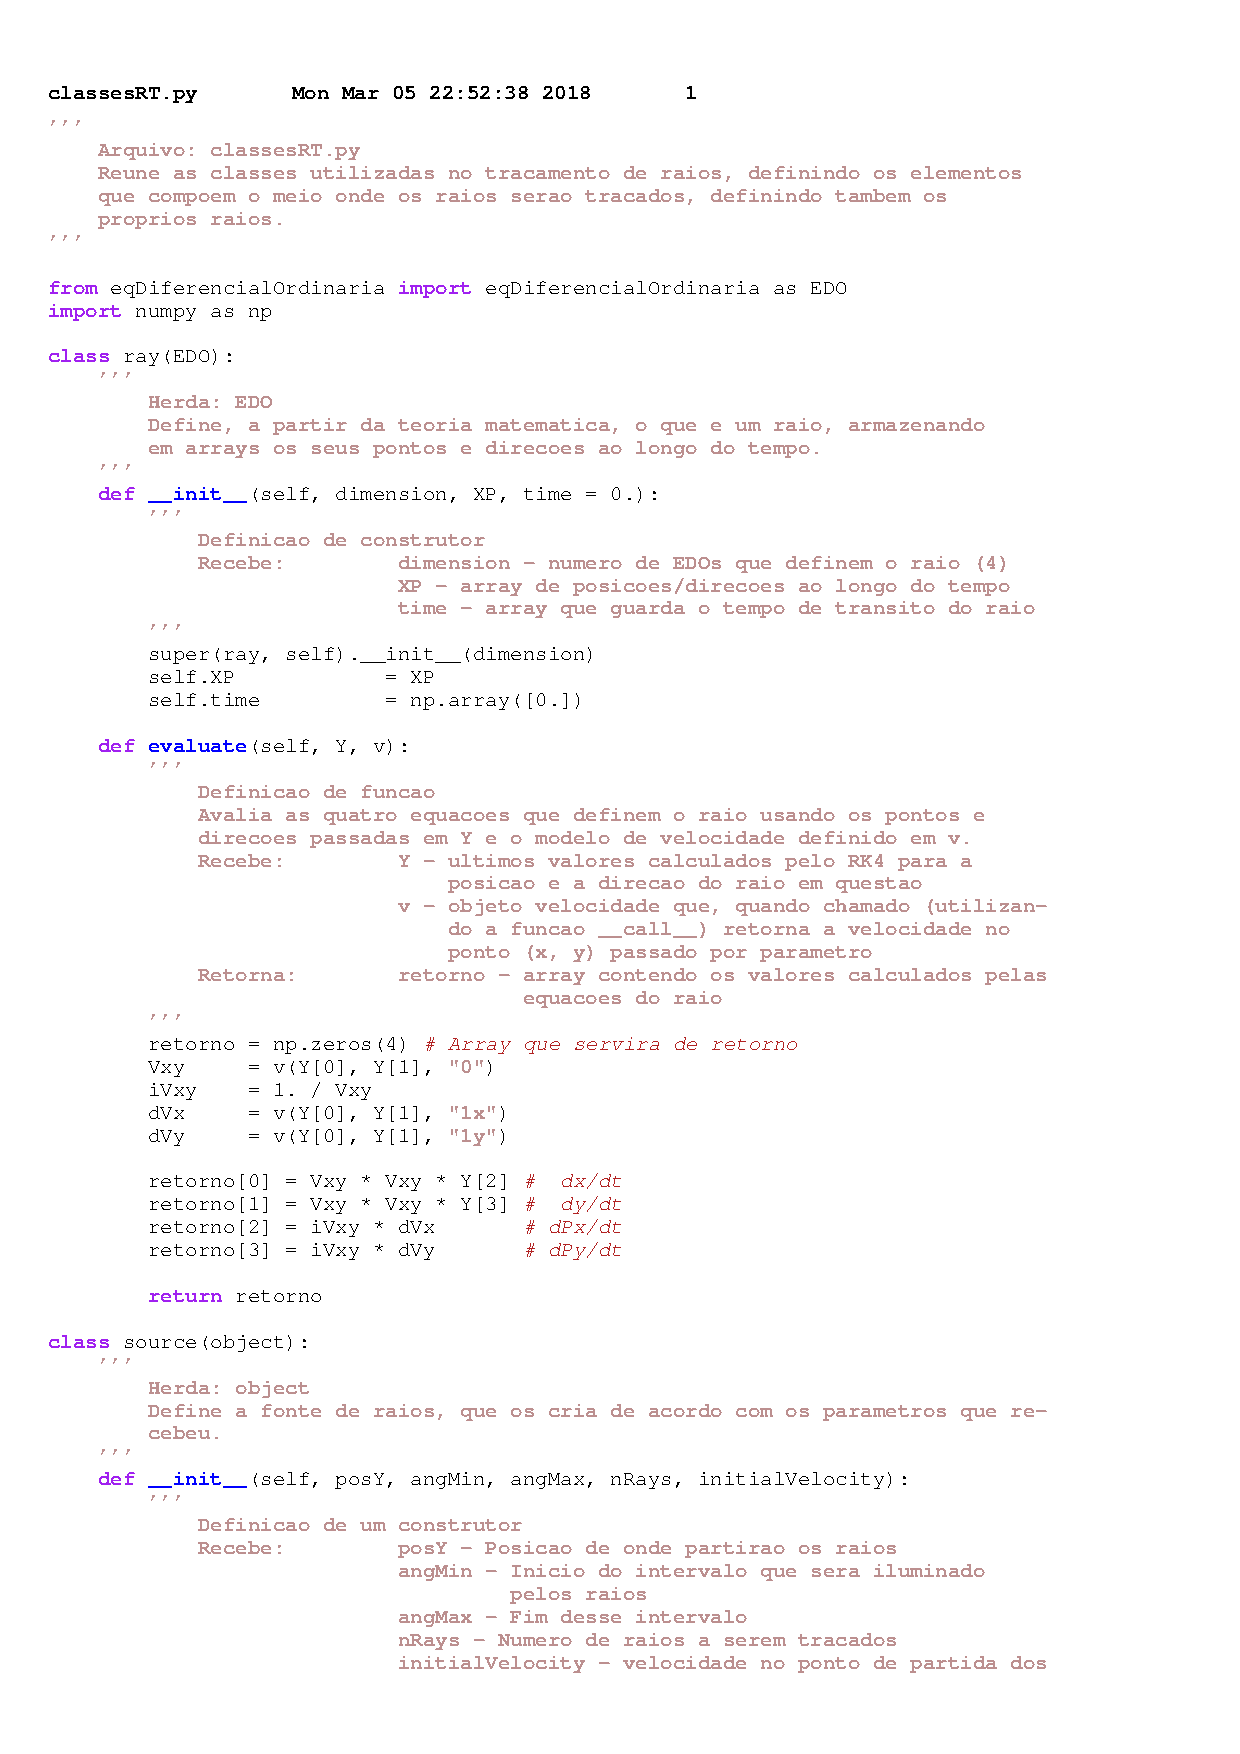
\includepdf[pages=-]{Codigos/RT/RT.pdf}
    \end{appendices}
    
    % Definindo o estilo de bibliografia
	\bibliographystyle{abbrv}
	
	% Definindo o arquivo .bib de bibliografia
	\bibliography{BIB}

\end{document}